\chapter{Identification of Strongly Connected Subsystems (SCSs) for Effective UQ}
\label{chap:scs}

\section{Proposed Framework for Identification of SCSs}
\label{scs_framework}

In this section, the main components of our proposed framework for SCS identification are outlined. The fundamental idea is to show how a large dimensional dynamical system can be decomposed into small interconnected subsystems (Figure~\ref{clusters_2}) to be solved in parallel. Figure~\ref{framework_fig} depicts the computational pipeline of the underlying methodology. Similar to WCS identification methodology~\cite{mukherjee2015laplacian,mukherjeecomparison} developed in Chapter~\ref{chap:wcs}, a graph-theoretic representation is adopted for a given dynamical system with involved uncertainty. Unlike the WCS identification approach, the graph is hypothesized to comprise of both weak and strong edges or couplings. The statistical linearization method is used to linearize the dynamical system in the domain of interest represented by the initial state density function (Figure~\ref{framework_fig}a). Next, a suitable overlapping community detection algorithm is applied to detect the SCSs (Figure~\ref{framework_fig}b). These SCSs determine the assignment of each node or variable to a cluster and their participation (Figure~\ref{framework_fig}c). The stochastic dynamical system corresponding to each SCS of reduced order is then propagated by a UQ method (Figure~\ref{framework_fig}d). An element-to-element product based step is applied to estimate the statistical properties of the state vector from the properties of the SCSs. These steps are followed to approximate the statistical properties, that is being propagated through the dynamics of the overall system. The overall procedure is continued till a measurement data is available. The measurement is used to filter out noise from the state variable, and the statistical properties are recalibrated using a Filtering technique (Figure~\ref{framework_fig}e). The cluster structure or the SCSs is/are then recomputed based on the updated statistical properties. The whole process continues during the required time of analysis. In the subsequent subsections, the theoretical and algorithmic details of each of these steps are discussed. 

\begin{figure}[H]
\centering
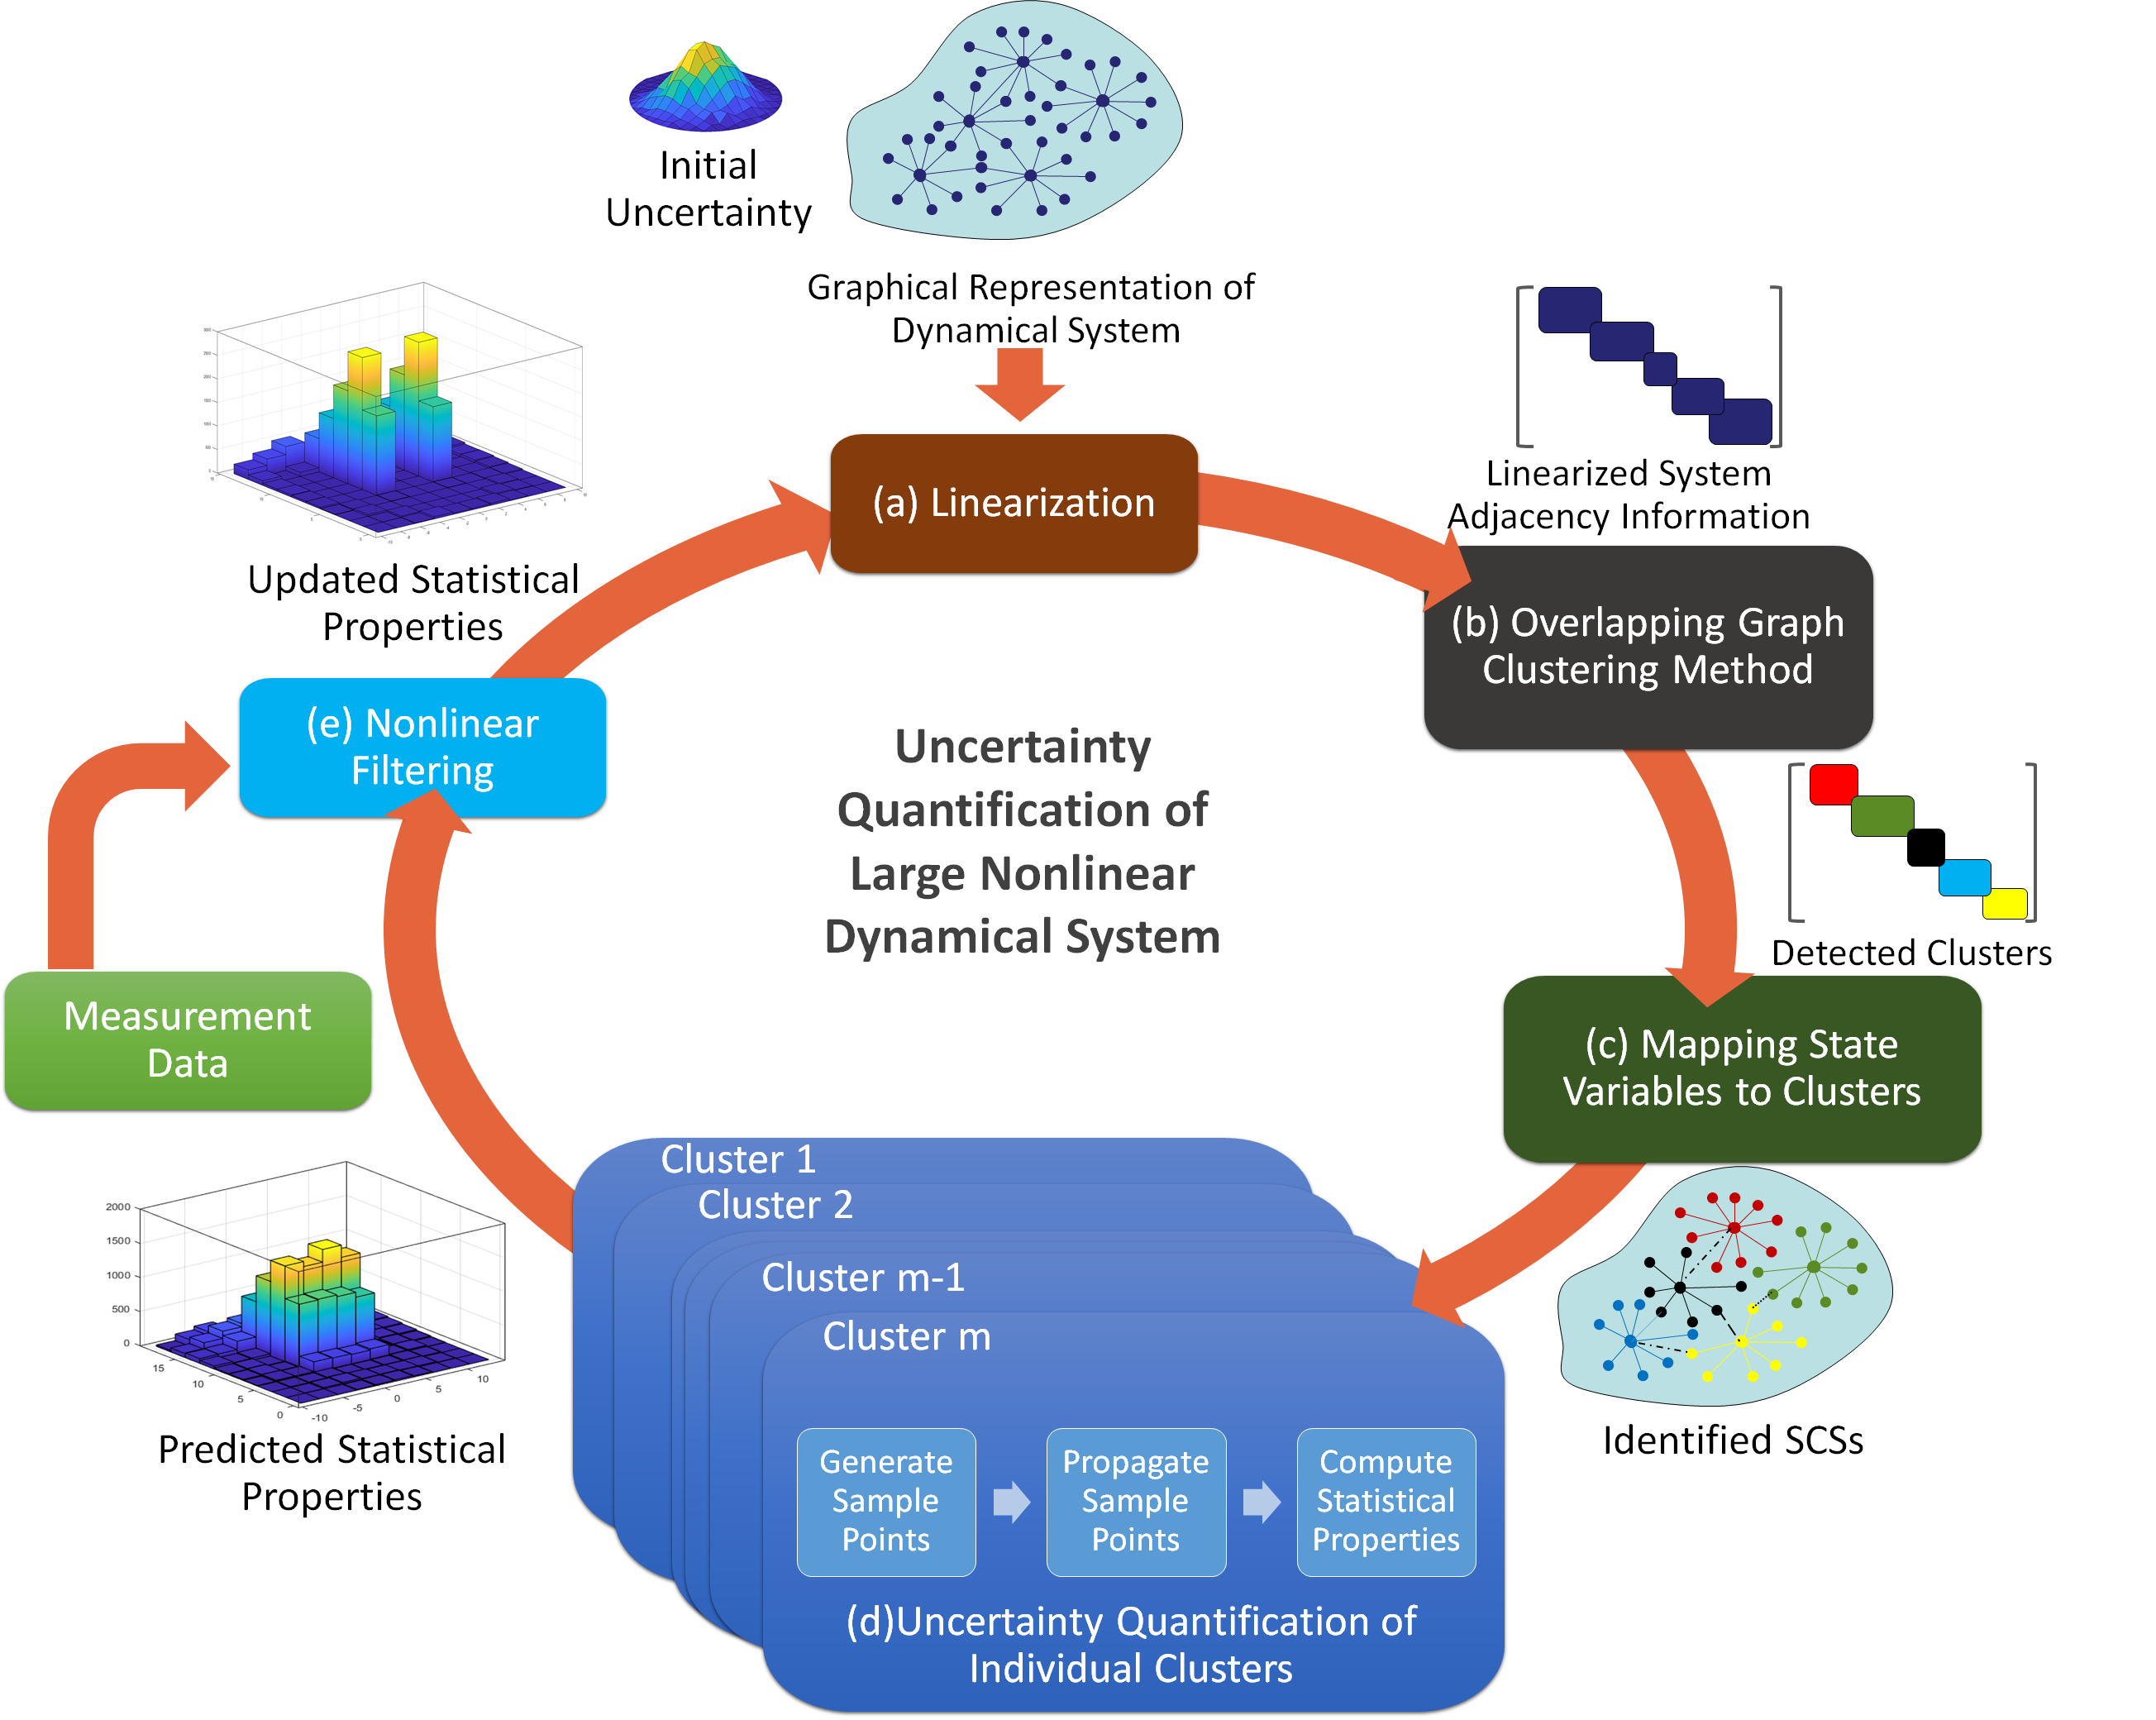
\includegraphics[scale=0.2]{figures_2/framework}
\caption{Overall Framework of the methodology}
\label{framework_fig}
\end{figure}

\section{Strongly Coupled Subsystems}

\newcommand{\bigCI}{\mathrel{\text{\scalebox{1.07}{$\perp\mkern-10mu\perp$}}}}
\newcommand{\nbigCI}{\centernot{\bigCI}}

\newcommand{\CI}{\mathrel{\perp\mspace{-10mu}\perp}}
\newcommand{\nCI}{\centernot{\CI}}

To define Strongly Connected Subsystem(SCS), a new state-space decomposition scheme is proposed with the following assumptions
\begin{itemize}
\item A state $x_i$, $i = 1$ to $n$, can participate in more than one cluster.
\item For each state, we quantify its association with a cluster. Instead of a binary $0-1$ association, we propose for a fuzzy association between 0 and 1. Such scheme can incorporate both decoupled and overlapping clusters.
%\item The association of a state with a cluster is also random.
\item The number of clusters is determined from the initial condition uncertainty and the associated dynamics for every run.
\end{itemize}

The association of the state $\textbf{x}$ in a particular cluster $j$ is defined by the variable $\textbf{z}_{j} \in \mathbb{R}^n$, $\textbf{z}_j = \lbrace z_{1j}, z_{2j},\ldots, z_{nj} \rbrace$, where $z_{ij}$, $i= 1$ to $n$ denotes the association of the state $x_i$ in cluster $j$. The variable $\textbf{z}$ has the following properties
\begin{itemize}
\item $\forall$ $i =1$ to $n$ and $j = 1$ to $m$, $0 \leq z_{ij} \leq 1$
\item $\sum_{j=1}^m z_{ij} = 1$
\end{itemize}

At each time instance, the state variable $\textbf{x}_t$ is represented in each cluster by the variable $\textbf{x}_t|j$ based on its association in a cluster $j$. A state $x_i$ having either 0, 1 (full) or partial association with a cluster. Thus, $x_i$ is represented by a linear combination of $x_{i}|j$'s, and its association $z_{ij}$, $j = 1$ to $m$ is given as,

\begin{equation}
\label{individual}
x_i = \sum_{j=1}^m  z_{ij} x_{i}|j
\end{equation}

\noindent In the vector notation the state vector is given as,

\begin{equation}
\label{main_frame}
\textbf{x}_t = \sum_{j=1}^m \textbf{z}_j \odot  \textbf{x}_t|j 
\end{equation} 

\noindent where, $\odot$ represents the element-to-element or Hadamard product and $\textbf{x}_t|j, \textbf{z}_j \in \mathbb{R}^{n}$ are $n$-dimensional random vectors. Also, for any two cluster $j_1$, $j_2 = 1$ to $m$, $j_1 \neq j_2$, we assume $\textbf{x}_t|j_1$ $\CI$ $\textbf{x}_t|j_2$. SCS or Strongly Connected Subsystem is therefore defined as the subset of $\textbf{x}_t|j$ for which $z_{ij} > \alpha$, where $\alpha$ is a very small threshold value. The values of $Z$ matrix ($Z = \lbrace z_{ij} \rbrace$) can be tabulated as shown in Table~\ref{zmatrix}.

\begin{table}[H]
\centering
\caption{The association values $z_{ij}$ tabulated in the matrix form}
\begin{tabular}{c|c|c|c|c}
\hline 
\backslashbox{States}{Clusters} & 1 & 2 & $\ldots$ & $m$ \\ 
\hline 
1 & $z_{11}$ & $z_{12}$ & \ldots & $z_{1m}$ \\  
2 & $z_{21}$ & $z_{22}$ & \ldots & $z_{2m}$ \\ 
$\vdots$ & $\ldots$ & $\ldots$ & $\vdots$ & $\ldots$ \\ 
$n$ & $z_{n1}$ & $z_{n2}$ & \ldots & $z_{nm}$ \\ 
\hline 
\end{tabular} 
\label{zmatrix}
\end{table}


The detailed theory and application of SCS for enabling UQ are discussed in subsequent subsections.


\subsection{Distribution of $\textbf{x}_t|j$}
\label{cluster_structure}

In this section, three methods for defining and estimating the statistical properties for $\textbf{x}|j$ and SCS are developed. SCS are determined as the subset $\textbf{x}_t^j|j \subset \textbf{x}|j$ for which the association in a cluster is greater than a very low threshold value. In other words $\textbf{x}_t^j|j = \lbrace x_i | z_{ij} > \alpha, i = 1 \text{ to } n \rbrace$, where $\alpha$ is the threshold parameter. In each cluster, the state variable $\textbf{x} \in \mathbb{R}^n$ into two disjoint unions $\textbf{x}_t^j|j \in \mathbb{R}^{n_j}$ and $\textbf{x}_t^{j'}|j \in \mathbb{R}^{n - n_j}$, where $\textbf{x}_t^{j}|j \cap \textbf{x}_t^{j'}|j = \emptyset $. All other association values $z_{ij}$ which are less than $\alpha$ are assumed to be 0. Under Hadamard product formulation in Equation~\ref{main_frame}, with 0 association value, the subset $\textbf{x}_t^{j'}|j$ does not contribute towards the distribution of $\textbf{x}_t$. The dynamics of the cluster $j$ evolve in the submanifold described by the reduced order subspace $\textbf{x}_t^{j}|j$ or the SCS similar to Equation~\ref{integral_wcs}. This decomposition technique facilitates the estimation of the statistical properties of SCSs and $\textbf{x}_t$ in parallel. 

 To have further ease in analysis, the concept of \textit{strong} and \textit{weak participants} have been developed. Three approximate models for $\textbf{x}_{t}^{j}|j$ have been proposed based on the participation of the subset $\textbf{x}_{\beta'}^{j}|j$ in clusters. Subsequently, the propagation equation and statistical properties for $\textbf{x}_{t}^{j}|j$ have been formulated under these approximations.
 
\subsubsection{Type I: Use of Hadamard Product}


In this approach, an SCS is defined as the set of variables  $\textbf{x}_t^j|j \in \mathbb{R}^{n_j}$ with $z_{ij} > \alpha $. By this definition, SCS has the following properties 
\begin{enumerate}
\item The state variable $\textbf{x}_t$ is a countable union of the SCSs. Thus $\bigcup _{j=1}^m \textbf{x}_t^j = \textbf{x}_t $
\item The intersection of two subsets is termed as the set of \textit{overlapping variables}. This set might not be an empty set.
\item The subsets are assumed to evolve under decoupled propagation equation and are statistically independent. Hence $\textbf{x}_t^{j_1} \CI \textbf{x}_t^{j_2}$ $\forall$ $j_1, j_1 = 1$ to $m$, $j_1 \neq _2$.   
\end{enumerate}
In each cluster, the submanifold $\textbf{x}_t^j$ for the SCS is defined by the following SDE,

\begin{equation}
\dot{\textbf{x}_t^j} = f_j(\textbf{x}_t^j)  
\end{equation}  

Thus, $m$ reduced order subsystems of order $n_j << n$ are solved instead of solving Equation~\ref{integral_whole}. Under this framework, the overlapping variables evolve with different propagation equation in different clusters. Finally, the approximate solution to Equation~\ref{moment_whole} and other statistical properties of $\textbf{x}_t$ are computed using the results from different clusters through the Hadamard product formulation (outlined in Section~\ref{hadamard_statistics}). The process of mapping state variables to overlapping clusters is shown in Figure~\ref{framework_TypeI}. 

\begin{figure}[H]
\begin{center}
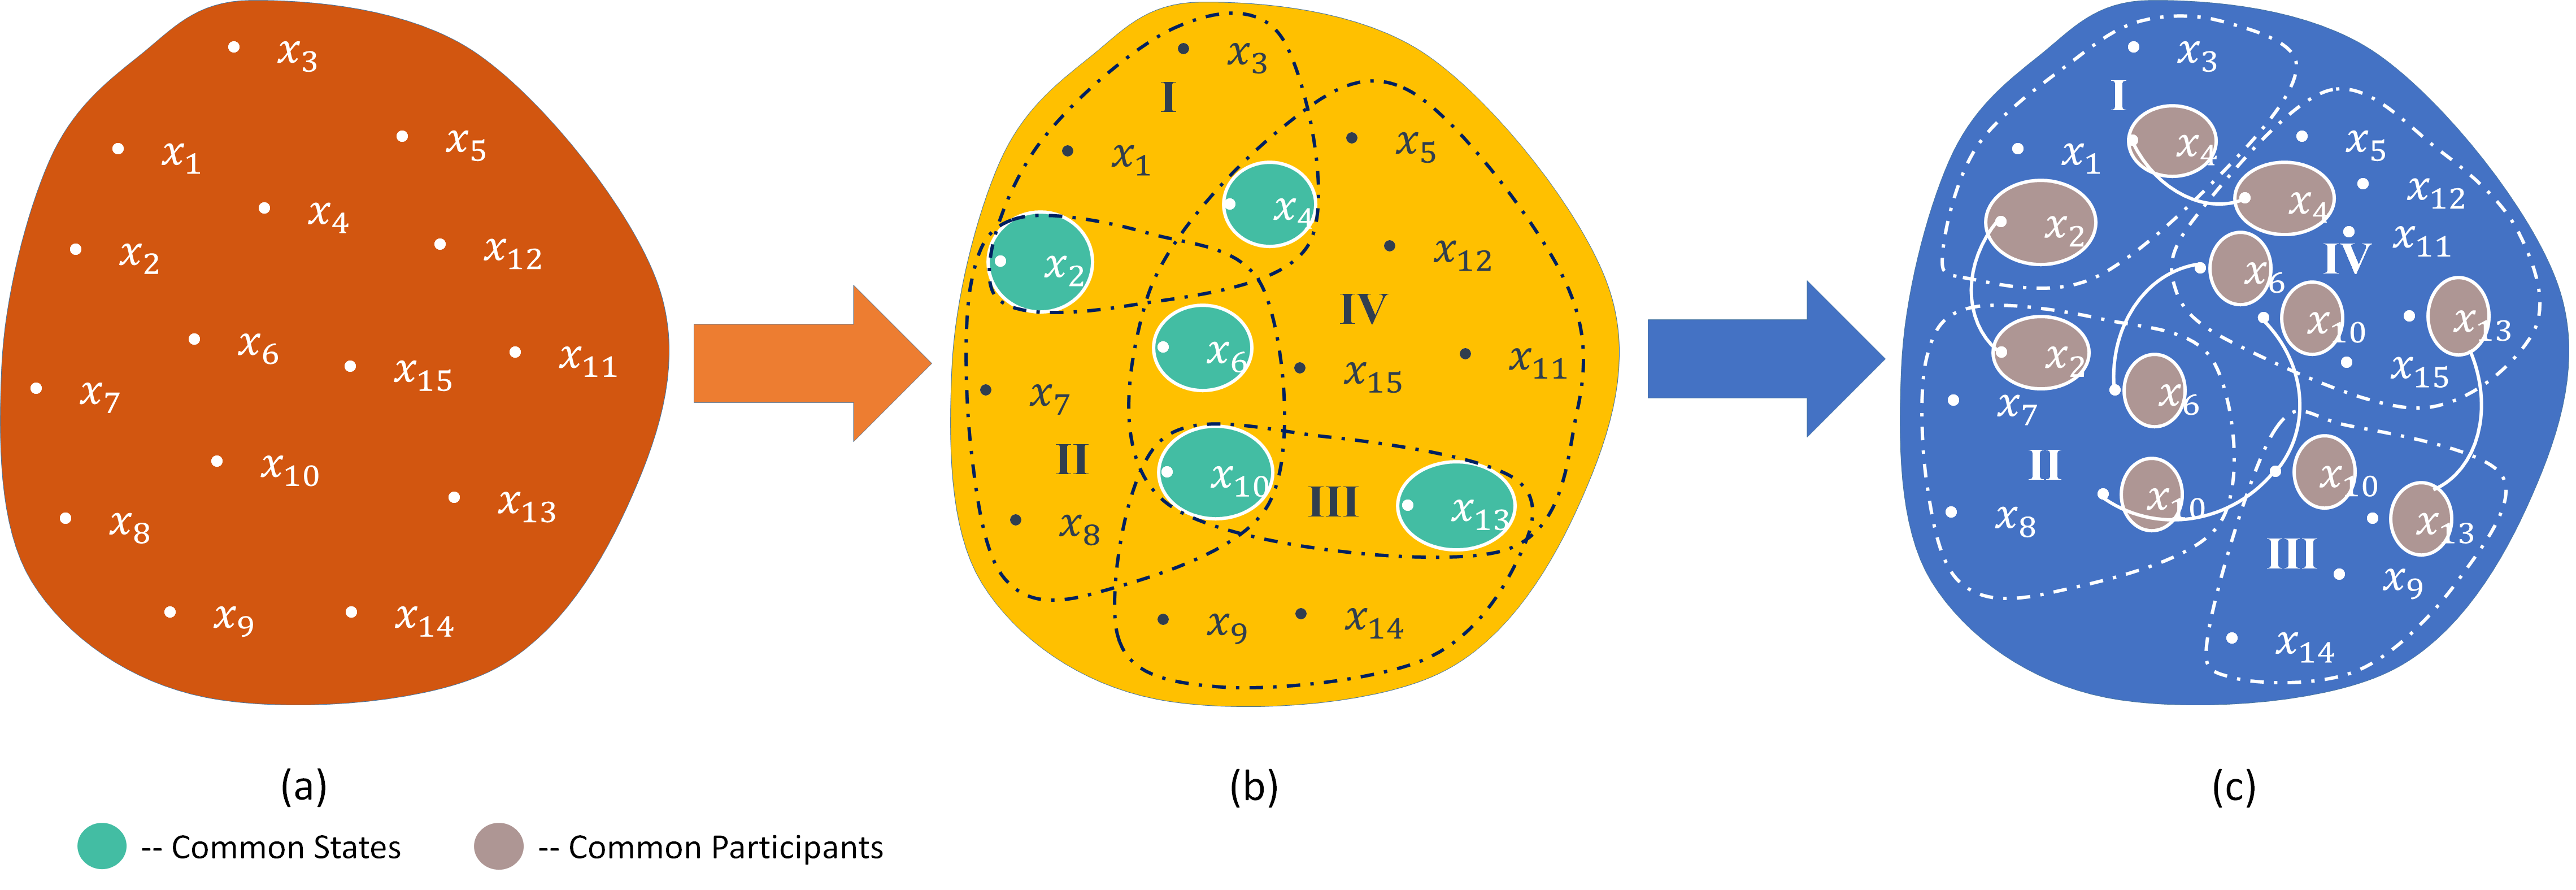
\includegraphics[width=\textwidth]{figures_2/TypeI}
\caption{Overall Framework of the Type I method of clustering: (a) Overall state-space domain (b) Identification of overlapping clusters (common states encircled) and (c) States being mapped to non-overlapping clusters with common states participating in more than one cluster with same initial condition.}
\label{framework_TypeI}
\end{center}
\end{figure}


\subsubsection{Type II: Identification of strong and weak participants}
\label{type_II}

In this approach, we assume a higher threshold value $\beta$, with $\beta > \alpha$. This decides the level of participation of $\textbf{x}_t^{j}|j$ in the cluster $j$. We further break the subset $\textbf{x}_j|j$ into two unions $\textbf{x}_{\beta}^{j}|j \in \mathbb{R}^{n_{j_\beta}}$ and $\textbf{x}_{\beta'}^{j}|j \in \mathbb{R}^{n_j - n_{j_\beta}}$, with $\textbf{x}_{\beta}^{j}|j \cap \textbf{x}_{\beta'}^{j}|j = \emptyset$. The subset $\textbf{x}_{\beta}^{j}|j = \lbrace x_i | z_{ij} > \beta, i = 1 \text{ to } n_j \rbrace$ is labeled as the set of \textit{strong participants} and the other subset $\textbf{x}_{\beta'}^{j}|j$ as the set of \textit{weak participants}. We assume the initial distribution for $\textbf{x}_j^{\beta'}|j$ and the subset is provided to the propagation equation for $\textbf{x}_j^{\beta'}|j$ as an input variable. While the properties of $\textbf{x}^j_t$ remain the same as that in Type I, the properties of the subsets $\textbf{x}_{\beta}^{j}|j$'s are different:
\begin{enumerate}
\item The union of the subsets $\textbf{x}_{\beta}^{j}|j$'s may not be equal to $\textbf{x}_t$.
\item The intersection of two subsets $\textbf{x}_{\beta}^{j}|j$'s is termed as the set of \textit{overlapping variables}. This set might not be an empty set. The overlapping variables are propagated in the same way as in Type I.
\item The subsets are assumed to evolve under decoupled propagation equation and are statistically independent. Hence $\textbf{x}_{\beta}^{j_1}|j_1 \CI \textbf{x}_{\beta}^{j_2}|j_2$ $\forall$ $j_1, j_1 = 1$ to $m$, $j_1 \neq _2$. 
\end{enumerate}
 The propagation equation for $\textbf{x}_{\beta}^{j}|j$ is thus:

\begin{equation}
d \textbf{x}_{\beta}^{j}|j = f_{j_\beta} (\textbf{x}_{\beta}^{j}|j, \textbf{x}_j^{\beta'}|j)dt 
\end{equation}

This is a reduced order system of order $n_{j_\beta} \leq n_j$. For the purpose of calculating the final mean and covariance, a modified association matrix $Z^s$ is constructed using the following steps:

\begin{enumerate}
\item Initialize $Z^s$ to $Z$. 
\item The associations of the weak participants are assumed to be 0 as $z^s_{ij} = 0 $ $\forall$ $z_{ij} < \beta$.
\item Each row $i$ of $Z^s$ is further normalized as $z_{ij}^s = z_{ij}^s/ \sum_{j = 1}^m z_{ij}^s$.
\end{enumerate}

Similar to Type I, the statistical properties of $\textbf{x}_t$ are computed using the results from different clusters and the modified association matrix derived from the Hadamard product formulation (outlined in Section~\ref{hadamard_statistics}). The process of mapping state variables to overlapping clusters is shown in Figure~\ref{framework_TypeII}. 

\begin{figure}[H]
\begin{center}
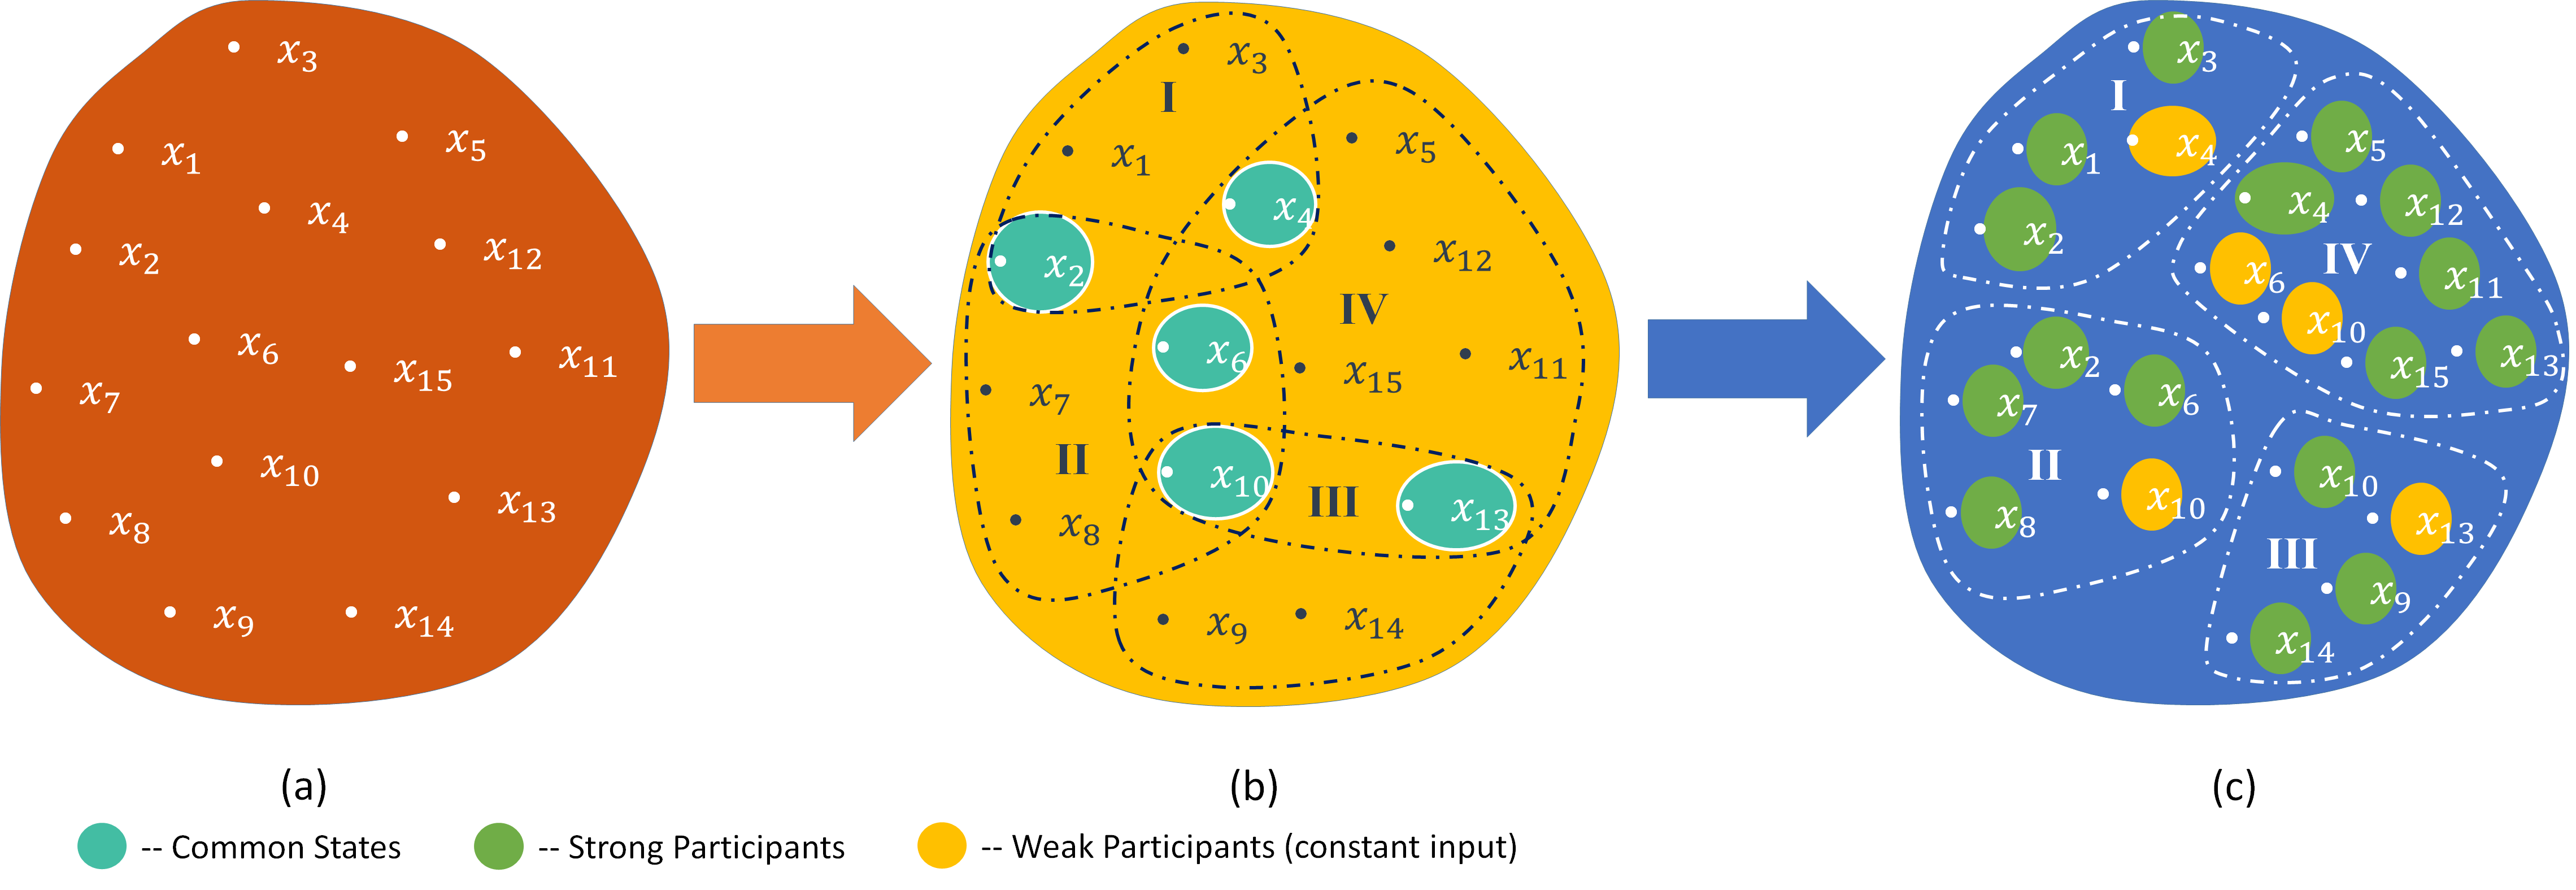
\includegraphics[width=\textwidth]{figures_2/TypeII}
\caption{Overall Framework of the Type II method of clustering: (a) Overall state-space domain (b) Identification of overlapping clusters (common states encircled) and (c) Identification of \textit{Strong} and \textit{Weak Participants}. \textit{Weak Participants} acting as constant input.}
\label{framework_TypeII}
\end{center}
\end{figure}

\subsubsection{Type III: Identifying Decoupled Subsystems}

This methodology is analytically similar to the method of identifying WCSs. A binary association matrix $Z^{decoup} \in \mathbb{R}^{n \times m}$ is constructed from the original matrix $Z$. In a row $i = 1$ to $n$ the maximum value of $z_{ij}$  is found out and is set to 1. The rest of the values are set to 0. This procedure gives us the $Z^{decoup}$ matrix. Thus, a state can participate in only one cluster and there is no overlap. The set $\textbf{x}^d_j|j \in \mathbb{R}^{n_d}$ contains only the states for which $z_{ij'}^{decoup} = 1$. Thus,
\begin{enumerate}
\item The subsets are disjoint partitions of $\textbf{x}_t$. This means $\bigcup _{j=1}^m \textbf{x}^d_j|j =\textbf{x}_t$ and $\textbf{x}^d_{j_1}|j_1 \CI \textbf{x}^d_{j_2}|j_1 = \emptyset$ $\forall$ $j_1, j_1 = 1$ to $m$, $j_1 \neq _2$. 
\item The subsets are decoupled and statistically independent. 
\end{enumerate}
Based on these assumptions, the submanifold $\textbf{x}_j^{d}|j$ is defined by the following SDE:

\begin{equation}
\dot{\textbf{x}}_j^{d}|j = f_j({\textbf{x}}_j^{d}|j)    \hspace{5 mm}  \textbf{x}_0 = {\textbf{x}}_j^{d}|j 
\end{equation}

The process of mapping state variables to overlapping clusters is shown in Figure~\ref{framework_TypeIII}. This is a reduced order system of order $n_d \leq n_{j_\beta} \leq n_j$. The next subsection discusses the numerical method for computing the association matrix $Z$ for the system defined in Equation~\ref{stochdyn}. 


\begin{figure}[H]
\begin{center}
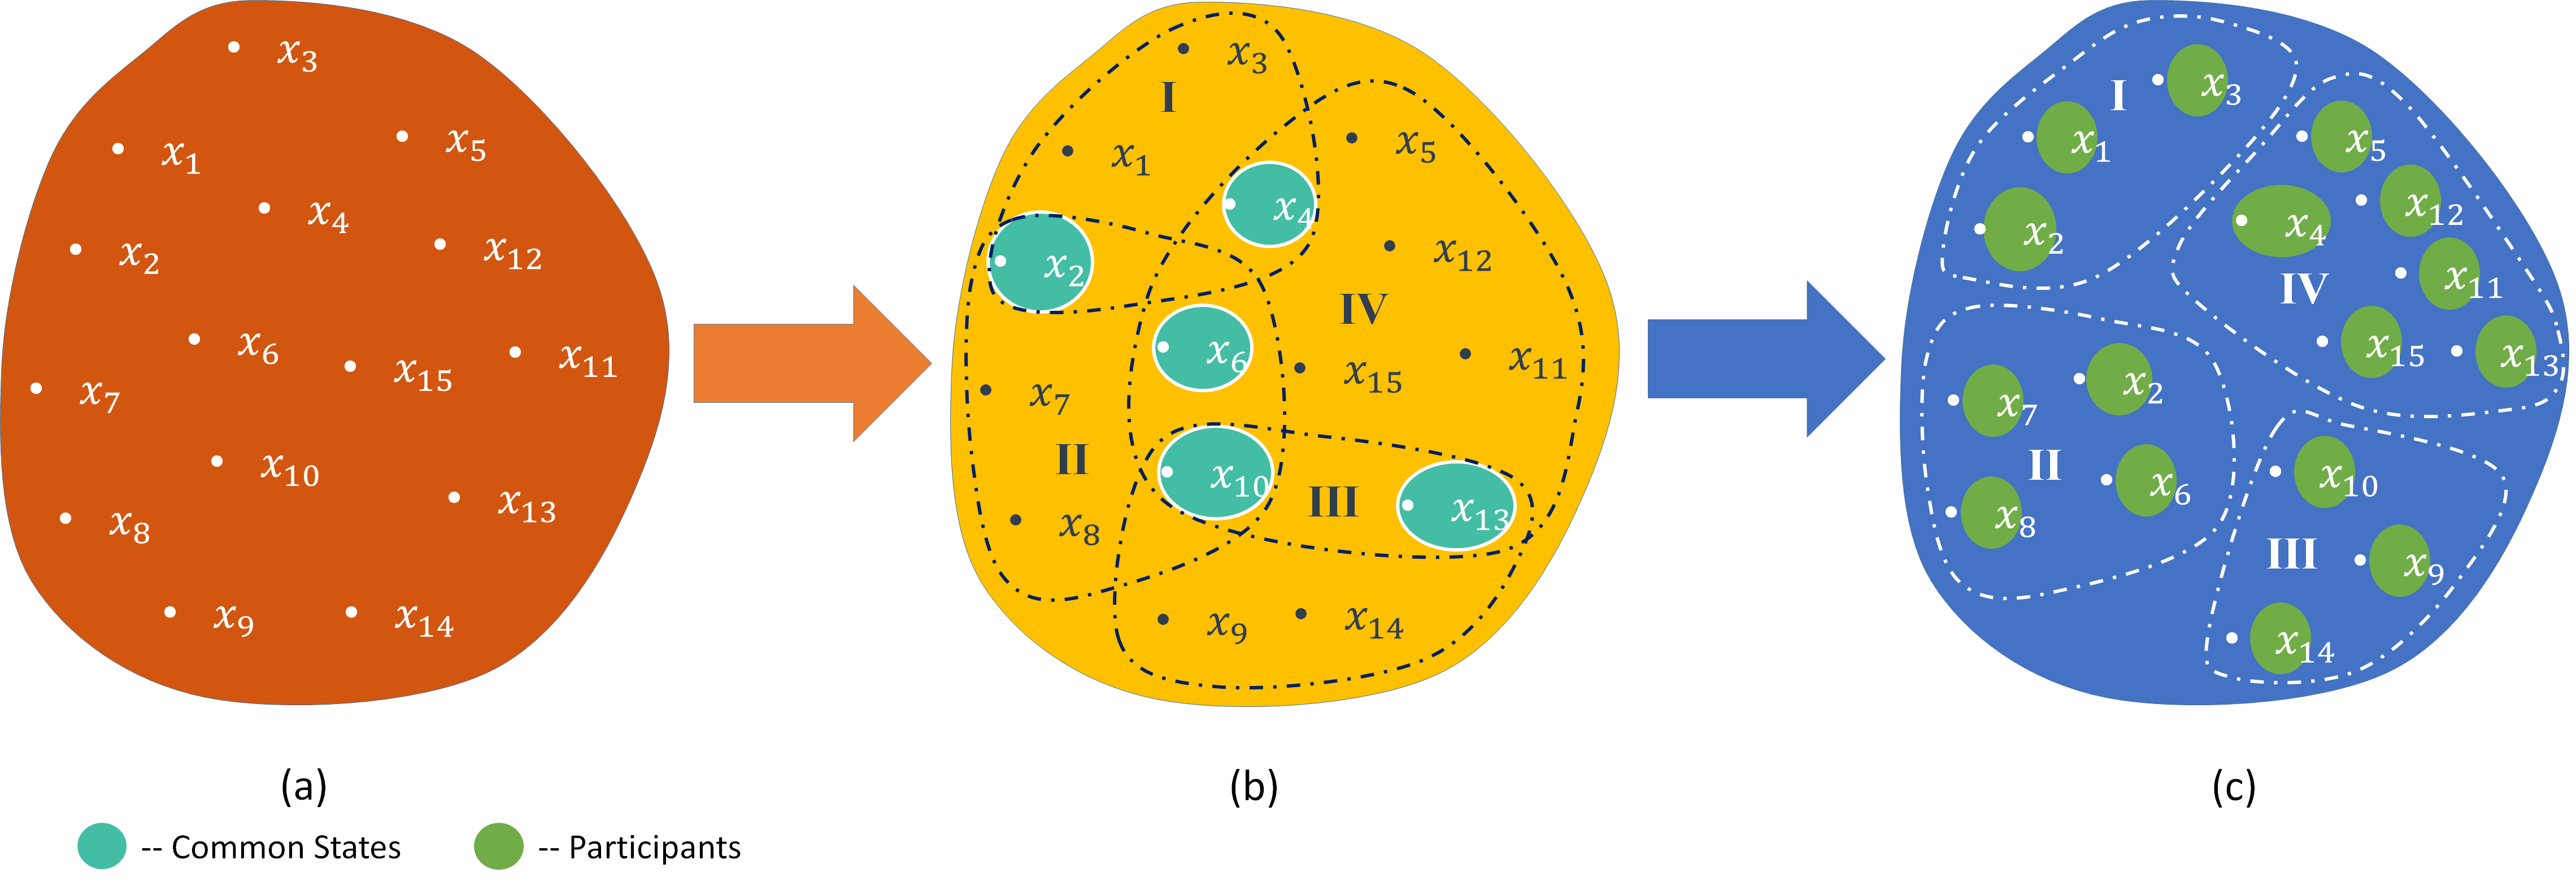
\includegraphics[width=\textwidth]{figures_2/TypeIII}
\caption{Overall Framework of the Type III method of clustering: (a) Overall state-space domain (b) Identification of overlapping clusters (common states encircled) and (c) Identification of non-overlapping clusters}
\label{framework_TypeIII}
\end{center}
\end{figure}


\section{Overlapping Graph Clustering}

The study of overlapping community has been a recent addition to the world of scientific research. Instead of detecting disjoint community in a network, in overlapping community framework, a node in a network can participate in multiple communities. In this context, Baumes \textit{et al.}~\cite{baumes2005finding} proposed a two-step algorithm to identify disjoint clusters, followed by an iterative method of assigning nodes to clusters till a density function is improved. Palla \textit{et al.} have developed a clique-based method and have applied the method to protein network comprising of 30,739 links~\cite{palla2005uncovering}. Algorithms such as LFM~\cite{lancichinetti2009detecting}, MONC~\cite{havemann2011identification}, CPMw~\cite{farkas2007weighted}, SCP~\cite{kumpula2008sequential} have extended the earlier work to enhance the applicability of community detection algorithms. OSLOM\cite{lancichinetti2011finding} and several effective overlapping community detection algorithms identifying overlapping cluster structures in complex networks also exist~\cite{shen2009detect,cazabet2010detection,padrol2010overlapping}. Although all the works mentioned above detect overlapping clusters, they do not quantify the degree of participation of a node in a given cluster. Fuzzy based clustering methods have been developed to address the shortcoming of quantifying the degree of participation. The \textit{fuzzy k-means} algorithm instead of optimizing the sum of the Euclidean distance between the nodes and the cluster centers, uses a weighted objective function is used to quantify the degree of participation~\cite{dunn1974well}. Zhang \textit{et al.}~\cite{zhang2007identification} has combined the fuzzy k-means clustering algorithm with the well-established method of Spectral Clustering~\cite{von2007tutorial}. Distribution based algorithms have been further developed, whereby the association of a node to a cluster is modeled as a probability distribution and is updated with the availability of the adjacency information~\cite{magdon2011ssde,latouche2011overlapping,psorakis2011overlapping}. In our current work, the Non-negative matrix factorization based algorithm to detect the degree of association of a node to a cluster~\cite{psorakis2011overlapping} have been used. This algorithm iteratively minimizes the rank of the degree matrix along with finding the association of the nodes in each cluster.


\section{Hadamard Product and Multivariate Statistics}
\label{hadamard_statistics}

%Let us explore the statistical properties of the variable $\textbf{x}_t$. First, we formulate the moments for an individual state variable $x_i$. As explained earlier, the state variable can be decomposed into independent clusters with degrees of association as given in Equation~\ref{individual} and \ref{main_frame}.   

Once the statistical properties of the SCSs are determined from the propagation and moment equations as given in Section~\ref{cluster_structure}, the first and second order moments for a state variable $x_i$  under the formulation of Equation~\ref{individual} is given as:

\begin{equation}
E \left[x_i \right] = E \left[ \sum_{j=1}^m z_{ij} x_{i}|j \right] =\sum_{j=1}^m  z_{ij} E \left[  x_{i}|j  \right]  
\end{equation}

and,

\begin{equation}
E \left[x_i^2 \right] = E \left[ \left( \sum_{j=1}^m z_{ij} x_{i}|j  \right)^2 \right] =\sum_{j=1}^m  z_{ij}^2 E \left[  x^2_{i}|j  \right]  + \sum_{j=1}^{m-1} \sum_{k=j+1}^m z_{ij}z_{ik}  E \left[  x_{i}|j  \right] E \left[  x_{i}|k  \right]
\end{equation}

Thus, the covariance formulation is given as: 

\begin{equation}
\mathbf{var}(x_i) = \sum_{j=1}^m z^2_{ij} \mathbf{var} (x_{i})
\end{equation}



\noindent Similarly, a general expression for any $\alpha^{\text{th}}$ order moment can be written using multinomial expansion as:

\begin{equation}
\begin{array}{ll}
E \left[x_i^{\alpha} \right] = \displaystyle E \left[ \left( \sum_{j=1}^m z_{ij} x_{i}|j  \right)^{\alpha} \right] &= \displaystyle E \left[ \sum_{k_1 + k_2 + \ldots + k_m = \alpha} \begin{pmatrix}
\alpha \\ k_1,k_2,\ldots,k_m
\end{pmatrix}  \prod_{1 \leq j \leq m} x^{k_j}_{i}|j  \; z^{k_j}_{ij} \right] \\
&= \displaystyle  \sum_{k_1 + k_2 + \ldots + k_m = \alpha} \begin{pmatrix}
\alpha \\ k_1,k_2,\ldots,k_m
\end{pmatrix}  \prod_{1 \leq j \leq m} z^{k_j}_{ij} \prod_{1 \leq j \leq m} E \left[ x^{k_j}_{i}|j \right]
\end{array}
\end{equation}

For the state vector $\textbf{x}_t$, the moment equations for the first two order under the formulation of Equation~\ref{main_frame} are given as:

\begin{equation}
\label{mean}
E \left[\textbf{x}_t \right] = E \left[ \sum_{j=1}^m \textbf{z}_j \odot \textbf{x}_t|j  \right] =\sum_{j=1}^m  \textbf{z}_j \odot E \left[  \textbf{x}_t|j  \right]  
\end{equation}

and,

\begin{equation}
\begin{array}{ll}
E \left[\textbf{x}_t \textbf{x}^T_t  \right] &= \displaystyle  \sum_{j=1}^m E \left[\left( \textbf{z}_j \odot \textbf{x}_t|j\right) \left( \textbf{z}_j \odot \textbf{x}_t|j\right)^T \right] + \sum_{j=1}^{m-1} \sum_{k=j+1}^m E \left[\left( \textbf{z}_j \odot \textbf{x}_t|j\right) \left( \textbf{z}_k \odot \textbf{x}_t|k\right)^T \right] \\
&= \displaystyle \sum_{j=1}^m \left( \textbf{z}_j \textbf{z}^T_j  \right) \odot E \left[ {\textbf{x}_t|j} \; {\textbf{x}_t|j}^T \right] + \sum_{j=1}^{m-1} \sum_{k=j+1}^m \left( \textbf{z}_j \textbf{z}^T_k  \right) \odot E \left[ {\textbf{x}_t|j}\right] E \left[{\textbf{x}_t|k} \right]^T
\end{array}
\end{equation}

Thus, the covariance matrix is given as:

\begin{equation}
\label{covariance}
\mathbf{cov}(\textbf{x}_t) = \sum_{j=1}^m \left(\textbf{z}_j \textbf{z}^T_j \right) \odot \mathbf{cov} \left( \textbf{x}_t|j \right)
\end{equation}

Furthermore, the moment generating function (mgf) for $x_i$ can be written as:

\begin{equation}
\begin{array}{ll}
M_{x_i}(\tau) &=  E \left[ e^{\tau x_i} \right] = E \left[ e^{\tau \sum_{j=1}^m  z_{ij} x_{i}|j} \right] = \displaystyle \prod_{j=1}^m E \left[e^{\tau (z_{ij} x_{i}|j )}  \right] \\
&= \displaystyle \prod_{j=1}^m M_{x_{i}|j} (z_{ij} \tau)
\end{array}
\end{equation}

Hence, the mgf of $\textbf{x}_t$ is given as:


\begin{equation}
\begin{array}{ll}
M_{\textbf{x}_t}(\bm{\tau}) &=  E \left[ e^{\bm{\tau}^T \textbf{x}_t} \right] =  E \left[ e^{\bm{\tau}^T \sum_{j=1}^m  \textbf{z}_j \odot \textbf{x}_t|j }  \right] = \displaystyle \prod_{j=1}^m E \left[e^{(\textbf{z}_j \odot \bm{\tau} )^T \textbf{x}_{t}|j }  \right] \\
&= \displaystyle \prod_{j=1}^m M_{\textbf{x}_t|j} (\textbf{z}_j \odot \bm{\tau})
\end{array}
\end{equation}

Equation~\ref{mean} and~\ref{covariance} have been used to estimate the statistical properties of the state variable $\textbf{x}$ obtained from the solution to Equation~\ref{integral_whole}. 

\section{Kalman Filter and Updating of Cluster Structure}
\label{ukf_clust}
In this section, the different subroutines are grouped to describe the overall framework. The linearization and clustering method described in Section~\ref{cluster_structure} is coupled with standard UQ method of Unscented Kalman Filter (UKF)~\cite{julier1997new} to analyze a high dimensional system defined in Chapter~\ref{chap:uq}. UKF has been the preferred method of UQ owing its speed and accuracy in estimating moments up to the second order of a Gaussian random vector by generating fewer sample points. 

% UKF proposes the following deterministic formulation for generating \textit{Sigma Points} from a Gaussian random variable $\textbf{x} \sim \mathcal{N}(\mu,\Sigma), \textbf{x} \in \mathbb{R}^n$,
% \begin{equation}
% \label{sigmapt}
% \begin{array}{lr}
% \mathcal{X}_0 = \mathbf{\mu} &W_0 = \kappa /(n+ \kappa)  \\
% \mathcal{X}_i = \mathbf{\mu} + \left( \sqrt{(n+ \kappa) \Sigma} \right)_i  &W_i = 1 /2(n+ \kappa)  \\
% \mathcal{X}_{i+n} = \mathbf{\mu} - \left( \sqrt{(n+ \kappa) \Sigma} \right)_i  &W_{i+n} = 1 /2(n+ \kappa)
% \end{array}
% \end{equation}
% \noindent $\left( \sqrt{(n+ \kappa) \Sigma} \right)_i$ is the $i$th row or column of the matrix square root of $(n+ \kappa) \Sigma$. These points accurately estimate the moment of $\textbf{x}$ up to the second order. These moment equations are given as,
% \begin{equation}
% \label{prop}
% \begin{array}{l}
% {\mu} =  \displaystyle \sum_{i=1}^{2n+1} W_i \mathcal{X}_i   \\
% \Sigma = \displaystyle \sum_{i=1}^{2n+1} W_i (\mathcal{X}_i - {\mu})(\mathcal{X}_i - {\mu})^T  \notag
% \end{array}
% \end{equation} 

Due to the coupling between the state variables, it is assumed that the cluster structure may change with time. Subsequently, there is a requirement of changing the cluster structure after a finite time evolution of the SCSs. This time is determined by the availability of measurement data. Measurements or observations are obtained from the actual running of the system at different time intervals. The measurement data is used to periodically update the statistical properties of the state variables using the UKF. The updated mean and covariance is used as the uncertainty information required to cluster the state space for the next finite time interval till the next measurement becomes available. All the methods mentioned above are combined to analyze a given large system. The different steps involved are as given below:

\begin{enumerate}
\item Given the problem 
\begin{equation}
\label{scs_meas_eqn}
\begin{array}{lr}
\dot{\textbf{x}}_t = f(\textbf{x}_t) & \textbf{x}_{t_0} = \textbf{x}_0 \\
\textbf{z}_t = \textbf{x}_t + \nu
\end{array}
\end{equation}
Where, $\textbf{z}_t$ is the measurement at a given time, and $\nu \sim \mathcal{N}(0,R_{\textbf{z}})$ is the measurement error.

\item At a time $t_0$, the nonlinear system is linearized as, 
\begin{equation}
f(\textbf{x}_{t_k}) = A_{sl}\textbf{x}_{t_k} + b_{sl}
\end{equation}
and clustered as per methods described in Section~\ref{cluster_structure}. At the end of this step, the number of subgroups or clusters in the state variables is identified, along with the association matrix $Z$ as given in Table~\ref{zmatrix}. 

\item The state-space is decomposed into SCS from the values of the association matrix $Z$ using the three methods of mapping described in Section~\ref{cluster_structure}.

\item Sigma points are generated using Equation~\ref{sigmapt} from the reduced order SCSs. The submanifold for each SCS is propagated as described in Section~\ref{cluster_structure} up to a certain time $t_k$. The mean and covariance for each SCS are estimated using Equation~\ref{prop}.

\item Once, the UQ of all the SCSs is complete, the mean and covariance of $\textbf{x}_{t_k}$ are computed using Equation~\ref{mean} and~\ref{covariance}.

\item Step 4 and 5 are continued up to a time $t_k + h$ till a measurement $\textbf{z}_{t_k + h}$ is available. Once a measurement update is available, the mean and covariance values are updated using the following steps of the UKF

\begin{enumerate}
\item The innovation covariance is then computed as:
\begin{equation}
P_{\nu \nu} = R_{\textbf{z}} + P_{k+h|k+h-1}
\end{equation}
\item The cross correlation matrix is computed as $P_{k+h|k+h-1}$
\item The Kalman gain is computed as: 
\begin{equation}
K = P_{k+h|k+h-1} P_{\nu \nu}^{-1}
\end{equation}
\item The measurement update is carried out:
\begin{equation}
\begin{array}{l}
\mu_{k+h|k+h} = \mu_{k+h|k+h-1} + K(\textbf{z}_{t_k + h} - \mu_{k+h|k+h-1})  \\
P_{k+h|k+h} = P_{k+h|k+h-1} - K P_{\nu \nu} K^T
\end{array}
\end{equation}

\item The above-defined recalibration of mean and covariance helps in updating the cluster structure of $\textbf{x}$. Using the updated statistical properties and the velocity function $f(\cdot)$, the association matrix $Z$ is recomputed using the methods described in Section~\ref{cluster_structure}. The state variables are further mapped into clusters using the three methods of mapping (Section~\ref{cluster_structure}). Steps 2-5 are repeated, and step 6 is used when a measurement becomes available. These steps are repeated iteratively till the whole analysis is complete.
\end{enumerate}


\end{enumerate}

\section{Three Coupled Lorenz Attractors}
\label{three_osc}
\subsection{The Problem Statement}

\begin{enumerate}
\item Coupled Lorenz Oscillators~\cite{lorenz1963deterministic},
\begin{equation}
\label{2d_lorenz}
\begin{array}{l}
\dot{x}_i = \sigma_i(y_i - x_i) +\epsilon(x_{i+1} - 2x_i + x_{i+1}) \\
\dot{y}_i = x_i (\rho_i - z_i) - y_i \\
\dot{z}_i = x_i y_i - \beta_i z_i \hspace{5mm} i = 1,2,3
\end{array}
\end{equation}
\item The coupling strength is $\epsilon = 1$. Other parameters are $\sigma_i = \begin{bmatrix} 8 & 9 & 12 \end{bmatrix}$, $\rho_i = \begin{bmatrix} 30 & 31 & 35 \end{bmatrix}$ and $\beta_i = \begin{bmatrix} 2.2432 & 2.9077 & 2.5923 \end{bmatrix}$
\item The measurement equation is $h = \textbf{x} + \nu$. Measurements are available from time 0 to $T = 10$ seconds at every $1$ second interval.
\item Initial distribution as $\textbf{x} \in \mathcal{N}(\bm{\mu}_{\textbf{x}},\Sigma_{\textbf{x}})$
\item Thresholds for clustering are $\alpha = 10^{-3}$ and $\beta = 0.1$
\end{enumerate}

\subsection{Association Matrix $Z$ at $t = 0$}

\begin{itemize}
\item From the initial distribution of $\textbf{x}_0$, generate $2n+1$ sigma points. These points are used to develop the statistically linearized matrix as given in Equation~\ref{stat_lin}.
\item The association matrix $Z = \begin{bmatrix}
z_{1} & z_2 & \ldots & z_m
\end{bmatrix} \in \mathbb{R}^{n \times m}$  is obtained by applying the Bayesian NMF on the matrix $A_{sl}$.
\item Any value in the matrix $Z$ less than $\epsilon_1$ is replaced by 0. The initial $Z$ matrix (Similar to Table~\ref{zmatrix}) for the problem is given in Table~\ref{init_zmatrix}. 
\newpage
\begin{table}[H]
\caption{Initial $Z$ matrix for Problem Statement in Equation~(\ref{2d_lorenz})}
\label{init_zmatrix}
\centering
\begin{tabular}{c|c|c|c}
\hline 
\backslashbox{States}{Clusters} & 1 & 2 & 3 \\ 
\hline
1 & 0.9474 & 0.0526 & 0 \\ 
2 & 1 & 0 & 0 \\ 
3 & 1 & 0 & 0 \\ 
4 & 0.0455 & 0.9091 & 0.0455 \\ 
5 & 0 & 1 & 0 \\ 
6 & 0 & 1 & 0 \\ 
7 & 0 & 0.0370 & 0.9630 \\ 
8 & 0 & 0 & 1 \\ 
9 & 0 & 0 & 1 \\ 
\hline 
\end{tabular} 
\end{table}
\end{itemize}

\subsection{Propagation Equation for $\textbf{x}_t$ using the three different approaches}

As discussed before, under the different type of models adopted, different cluster structures from the same association matrix are obtained. For analysis of the system up to the next available measurement, the three different models for time interval $[0,1]$ at every 0.01s have been simulated. 

\subsubsection{Type I Method}

Using Type I approach, the identified clusters are tabulated in Table~\ref{Type1_cluster_lorenz}.

\begin{table}[H]
\centering
\caption{State Space cluster for Type I method}
\label{Type1_cluster_lorenz}
\begin{tabular}{c|c|c}
\hline 
Cluster & $\textbf{x}_t^j|j$ & States \\
\hline 
1 & $\textbf{x}_t^1|1$ & $\lbrace x_1,y_1,z_1,x_2 \rbrace$ \\ 
2 & $\textbf{x}_t^2|2$ & $\lbrace x_1,x_2,y_2,z_2,x_3 \rbrace$  \\ 
3 & $\textbf{x}_t^3|3$ & $\lbrace x_2, x_3, y_3, z_3 \rbrace$ \\ 
\hline 
\end{tabular} 
\end{table}

The propagation equation for each cluster involves only the states participating in the cluster. For example, the propagation equations for cluster 2 is given as follows:

\begin{equation}
\label{type1:lorenz}
\begin{array}{l}
\dot{x}_1 = -\sigma_1 x_1 +\epsilon(- 2x_1 + x_2) \\
\dot{x}_2 = \sigma_2(y_2 - x_2) +\epsilon(x_1 - 2x_2 + x_3) \\
\dot{y}_2 = x_2 (\rho_2 - z_2) - y_2 \\
\dot{z}_2 = x_2 y_2 - \beta_i z_2  \\
\dot{x}_3 = -\sigma_3 x_3 +\epsilon(x_2 - 2x_3) \\
\end{array}
\end{equation}

Equation~\ref{type1:lorenz} is a 5th order system of equation involving 5 random variables. Using UT, Equation~\ref{type1:lorenz} can be solved using $2 \times 5 + 1 = 11$ sigma points. The Mean and Covariance for $\textbf{x}_t$ are calculated using the Hadamard Product formulation (Equation~\ref{mean} and~\ref{covariance}). With the availability of measurement data, the mean and covariance are calibrated and the association matrix is updated as described in Step 6 in Section~\ref{ukf_clust}.

\subsubsection{Type II Method}
 
Using Type II approach, the identified \textit{strong and participant} subsets $\textbf{x}_{\beta}^{j}|j$ and $\textbf{x}_{\beta'}^{j}|j$ from the association matrix are listed in Table~\ref{Type2_cluster_lorenz},

\begin{table}[H]
\centering
\caption{State Space cluster for Type II method}
\label{Type2_cluster_lorenz}
\begin{tabular}{c|c|c|c|c}
\hline 
Cluster & $\textbf{x}_{\beta}^{j}|j$ & States & $\textbf{x}_{\beta'}^{j}|j$ & States \\ 
\hline
1 & $\textbf{x}_{0.1}^{1}|1$ & $\lbrace x_1,y_1,z_1 \rbrace$ & $\textbf{x}_{0.1'}^{1}|1$ & $ \lbrace x_2 \rbrace$ \\ 
2 & $\textbf{x}_{0.1}^{1}|1$ & $\lbrace x_2,y_2,z_2 \rbrace$ & $\textbf{x}_{0.1'}^{1}|1$ & $\lbrace x_1,x_3 \rbrace$ \\ 
3 & $\textbf{x}_{0.1}^{1}|1$ & $\lbrace x_2, x_3, y_3, z_3 \rbrace$  & $\textbf{x}_{0.1'}^{1}|1$ & $\lbrace x_3 \rbrace$ \\ 
\hline 
\end{tabular} 
\end{table}

For each cluster, the propagation equations will of the order of the subset $\textbf{x}_{\beta}^{j}|j$. The subset $\textbf{x}_{\beta'}^{j}|j$ acts as an input. The statistical properties of the input variable is same as that of $\textbf{x}_{\beta'}^{j}|j$ at time t= 0. According to Type II method, the propagation equations for the cluster 2 will be as follows:

\begin{equation}
\label{typeii_lorenz}
\begin{array}{l}
\dot{x}_2 = \sigma_2(y_2 - x_2) +\epsilon(u_1 - 2x_2 + u_3) \\
\dot{y}_2 = x_2 (\rho_2 - z_2) - y_2 \\
\dot{z}_2 = x_2 y_2 - \beta_i z_2 
\end{array}
\end{equation}

Here, $E[u_1] = E[x_1 (0)] $, $E[u_3] = E[x_3 (0)] $ and $E[u_1 u_1^T] = E[x_1 (0)x_1^T (0)] $, $E[u_3 u_3^T] = E[x_3 (0)x_3^T (0)] $. The overlapping variables evolve in those clusters only where it is has an association value more than the threshold parameter $\beta$. Also, the order of the propagation equations for cluster 2 in Type II method is less than that in Type I method. Lower order ensures faster estimation of the state variables of cluster 2 by the propagation equations in Type II method. Using UT, a 3rd order system equation for cluster 2 in Equation~\ref{typeii_lorenz} is solved using $2 \times 5 +1 = 11$ sigma points. The modified association matrix $Z^s$ for the purpose of calculation of statistical properties of $\textbf{x}_t$ is given in Table~\ref{Zs_matrix_lorenz}. 

\begin{table}[H]
\centering
\caption{$Z_s$ matrix for Type II method}
\label{Zs_matrix_lorenz}
\begin{tabular}{c|c|c|c}
\hline 
\backslashbox{States}{Clusters} & 1 & 2 & 3 \\ 
\hline
1 & 1 & 0 & 0 \\  
2 & 1 & 0 & 0 \\  
3 & 1 & 0 & 0 \\ 
4 & 0 & 1 & 0 \\ 
5 & 0 & 1 & 0 \\  
6 & 0 & 1 & 0 \\  
7 & 0 & 0 & 1 \\ 
8 & 0 & 0 & 1 \\  
9 & 0 & 0 & 1 \\ 
\hline 
\end{tabular} 
\end{table}

With the increase in the value of $\epsilon$ in Equation~\ref{2d_lorenz}, Type II method fails to identify \textit{strong and weak participants} separately for the same threshold value $\beta$. Thus, in problems with a high value of $\epsilon$, Type II and Type I yields the same cluster structure. 

\subsubsection{Type III Method}

In Type III method, the modified association matrix $Z^{decoup}$ is computed by keeping only the maximum value of $z_{ij}$ in a row and assuming the rest to be 0, followed by their row normalization. In the current problem defined in Equation~\ref{2d_lorenz}, the matrix  $Z^{decoup}$ is given as the $Z_s$ matrix in Table~\ref{Zs_matrix_lorenz}:

\newpage
%\begin{table}[h]
%\centering
%\begin{tabular}{|c|c|c|}
%\hline 
% 1 & 0 & 0 \\ 
%\hline 
%1 & 0 & 0 \\ 
%\hline 
%1 & 0 & 0 \\ 
%\hline 
%0 & 1 & 0 \\ 
%\hline 
%0 & 1 & 0 \\ 
%\hline 
%0 & 1 & 0 \\ 
%\hline 
%0 & 0 & 1 \\ 
%\hline 
%0 & 0 & 1 \\ 
%\hline 
%0 & 0 & 1 \\ 
%\hline 
%\end{tabular} 
%\end{table}

From the modified association matrix, the identified cluster structure and the variables belonging to each cluster are listed in Table~\ref{Type3_cluster_lorenz}.

\begin{table}[H]
\centering
\caption{State Space cluster for Type I method}
\label{Type3_cluster_lorenz}
\begin{tabular}{c|c|c}
\hline 
Cluster & $\textbf{x}^d_j|j$ & States \\
\hline 
1 & $\textbf{x}^d_1|1$ & $\lbrace x_1,y_1,z_1 \rbrace$ \\ 
2 & $\textbf{x}_d^2|2$ & $\lbrace x_2,y_2,z_2 \rbrace$  \\ 
3 & $\textbf{x}_d^3|3$ & $\lbrace x_3, y_3, z_3 \rbrace$ \\ 
\hline 
\end{tabular} 
\end{table}

The propagation equation for the decoupled subsets contains no overlapping variable. The equation for cluster 2 is as follows:

\begin{equation}
\label{type3_lorenz}
\begin{array}{l}
\dot{x}_2 = \sigma_2(y_2 - x_2) +\epsilon(- 2x_2) \\
\dot{y}_2 = x_2 (\rho_2 - z_2) - y_2 \\
\dot{z}_2 = x_2 y_2 - \beta_i z_2 
\end{array}
\end{equation}

Equation~\ref{type3_lorenz} is a 3rd order system involving three random variables. The required number of sigma points using UT is $2 \times 3 + 1 = 7$. This type of clustering is the least computationally expensive method. However, its performance degrades with the increase in coupling strength. 

\subsection{Results}

\begin{itemize}
\item The overall error in the estimation of mean is defined as:
\begin{equation}
\bar{e}_{\mu} = \frac{1}{nT} \left\lVert \frac{\mu_t - \hat{\mu}_t}{\mu_t} \right\rVert_2
\end{equation}
\item Figure~\ref{plot_9dim} shows the comparison of the original noisy and the noise free estimated trajectory.  
\end{itemize}

\begin{figure}[H]
\centering
\resizebox {\textwidth} {!} {
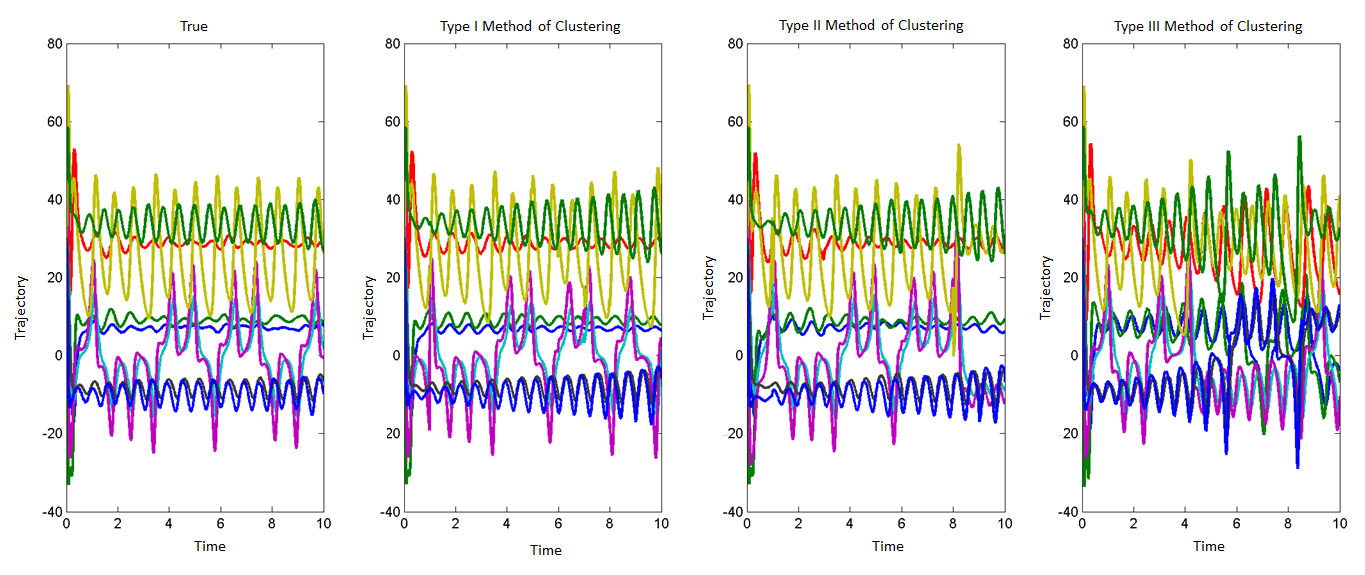
\includegraphics[scale=0.5]{figures_2/fig_comp_9dim}
}
\caption{Dimension $n= 9$, coupling strength $\epsilon= 1$}
\label{plot_9dim}
\end{figure} 


\section{Diffusively Coupled Lorenz Attractors}

The three coupled Lorenz Attractor problem in Section~\ref{three_osc} is further scaled to high dimensional systems. The equation of $N$ nonidentical and decoupled Lorenz attractors is defined by the following system of differential equation:  
\begin{equation}
\label{lorenz_coup}
\begin{array}{lc}
\dot{x}_{i} = \sigma_i (y_{i} - x_{i}) + \epsilon (x_{i+1} + x_{i-1} - 2x_{ti})  \\
\dot{y}_{i} = x_{i}(\rho_i - z_i) - y_{i} \\
\dot{z}_{i} = x_{i}y_{i} - \beta z_{i} & \hspace{5 mm}
i = 1,2,\ldots,N
\end{array} 
\end{equation} %\epsilon (x_{i+1} + x_{i-1} - 2x_{ti})

The system in Equation~\ref{lorenz_coup} is linearized and the state space is clustered following the methods described in Sections~\ref{cluster_structure} and~\ref{cluster_structure}.  Lorenz attractors exhibit chaotic properties for certain parameters. With $e = 0$, the equilibrium point for any set of parameters for an individual oscillator is $[0 \; 0 \; 0]^T$. With slight perturbation, the system repels from the equilibrium point and orients itself around two steady convection given by $\left( \pm\sqrt{\beta(\rho-1)}, \pm\sqrt{\beta(\rho-1)}, \rho-1 \right)$. To study the effectiveness of our proposed methodology, 42 test cases of the problem in Equation~\ref{lorenz_coup} are considered by taking seven values of $\epsilon = \lbrace 0.1, 1, 5, 10, 20, 50, 100 \rbrace$ and six values of $N =  \lbrace 5, 10, 25, 50, 100, 250  \rbrace $. Table~\ref{scs_weaklorenz} shows the average mean of error in propagation obtained for the three methods for some of the test cases. Lorenz system is a highly chaotic system. Hence, any slight error in wrong cluster detection can lead to an accumulation of significant error with time.

\begin{table}[H]
\caption{RMS \textit{time-averaged} mean for different test setups in Coupled Lorenz Oscillators}
\begin{center}
\resizebox{0.4\columnwidth}{!}{
\label{scs_weaklorenz}
\begin{tabular}{|c|c|c|c|c|}
\hline 
$N$ &   $\epsilon$ &   \multicolumn{3}{c|}{Type} \\ \hline
    &        &    1    &    2    &    3    \\ \hline
5    &    1    &    0.0135    &    0.0256    &    1.1243    \\ \hline
    &    20    &    0.0152    &    0.0360    &    0.3811    \\ \hline
    &    50    &    0.0175    &    0.0364    &    0.1008    \\ \hline
    &    100    &    0.0255    &    0.0386    &    0.0402    \\ \hline
10    &    0.1    &    0.0076    &    0.0093    &    3.3198    \\ \hline
    &    1    &    0.0077    &    0.0128    &    2.7919    \\ \hline
    &    5    &    0.0114    &    0.0165    &    0.8261    \\ \hline
    &    10    &    0.0106    &    0.0181    &    0.5274    \\ \hline
    &    20    &    0.0152    &    0.0188    &    0.1333    \\ \hline
25    &    0.1    &    0.0037    &    0.0043    &    1.3346    \\ \hline
    &    1    &    0.0036    &    0.0055    &    0.8408    \\ \hline
    &    5    &    0.0052    &    0.0066    &    0.1862    \\ \hline
    &    10    &    0.0051    &    0.0072    &    0.2684    \\ \hline
    &    20    &    0.0041    &    0.0074    &    0.1083    \\ \hline
    &    50    &    0.0057    &    0.0076    &    0.0234    \\ \hline
    &    100    &    0.0077    &    0.0098    &    0.0106    \\ \hline
50    &    1    &    0.0021    &    0.0028    &    0.6497    \\ \hline
    &    5    &    0.0000    &    0.0026    &    0.0033    \\ \hline
    &    10    &    0.0000    &    0.0036    &    0.0041    \\ \hline
    &    100    &    0.0039    &    0.0054    &    0.0136    \\ \hline
100    &    0.1    &    0.0009    &    0.0011    &    1.2278    \\ \hline
    &    1    &    0.0000    &    0.0009    &    0.0014    \\ \hline
    &    5    &    0.0000    &    0.0013    &    0.0017    \\ \hline
    &    10    &    0.0000    &    0.0013    &    0.0018    \\ \hline
    &    20    &    0.0019    &    0.0071    &    0.0608    \\ \hline
    &    50    &    0.0019    &    0.0058    &    0.1974    \\ \hline
\end{tabular} 
}
\end{center}
\end{table}

\section{Diffusively Coupled Van der Pol Oscillators}
The state space equations of weakly coupled Van der Pol Oscillators is given as~\cite{van1920theory}:

\begin{equation}
\label{strong_vanderpol}
\begin{array}{l}
\dot{x}_i = y_i + \epsilon (x_{i-1} - 2x_i + x_{i+1}) \\
\dot{y}_i = \mu(1-x_i^2)y_i - x_i  
\end{array}\hspace{5 mm} i = 1,2,\ldots,N
\end{equation}

The value of the $\epsilon$ is kept very low to introduce a weak coupling between the oscillators. Strong coupling induces a change in the behavior of the individual oscillator. The changing cluster structure needs to be identified with time to avoid accumulation of error. Table~\ref{strongvanderpol} shows the average mean of error in propagation obtained for the three methods for some of the test cases.

\begin{table}[H]
\caption{RMS \textit{time-averaged} mean for different test setups in Coupled Van der Pol Oscillators}
\begin{center}
\resizebox{0.4\columnwidth}{!}{
\label{strongvanderpol}
\begin{tabular}{|c|c|c|c|c|}
\hline 
$N$ &   $\epsilon$ &   \multicolumn{3}{c|}{Type} \\ \hline
    &        &    1    &    2    &    3    \\ \hline
5    &    0.1    &    0.00190    &    0.0023    &    0.00279    \\ \hline
    &    1    &    0.00339    &    0.0179    &    0.02887    \\ \hline
    &    5    &    0.00323    &    0.0075    &    0.03404    \\ \hline
10    &    0.1    &    0.00082    &    0.0012    &    0.00126    \\ \hline
    &    1    &    0.00473    &    0.0079    &    0.01142    \\ \hline
    &    5    &    0.01282    &    0.0152    &    0.02383    \\ \hline
    &    20    &    0.01937    &    0.0215    &    0.02645    \\ \hline
    &    100    &    0.02112    &    0.0228    &    0.02428    \\ \hline
25    &    0.1    &    0.00046    &    0.0006    &    0.00103    \\ \hline
    &    10    &    0.01053    &    0.0107    &    0.01106    \\ \hline
    &    20    &    0.01096    &    0.0117    &    0.01271    \\ \hline
    &    50    &    0.01131    &    0.0128    &    0.01315    \\ \hline
50    &    0.1    &    0.00028    &    0.0003    &    0.00052    \\ \hline
    &    1    &    0.00153    &    0.0032    &    0.00387    \\ \hline
    &    5    &    0.00394    &    0.0049    &    0.00492    \\ \hline
    &    10    &    0.00519    &    0.0052    &    0.00558    \\ \hline
    &    20    &    0.00539    &    0.0060    &    0.00647    \\ \hline
    &    50    &    0.00558    &    0.0068    &    0.00689    \\ \hline
100    &    1    &    0.00072    &    0.0015    &    0.00178    \\ \hline
    &    5    &    0.00187    &    0.0023    &    0.00253    \\ \hline
    &    10    &    0.00241    &    0.0026    &    0.00271    \\ \hline
    &    50    &    0.00260    &    0.0036    &    0.00383    \\ \hline
    &    100    &    0.00264    &    0.0038    &    0.00415    \\ \hline
250    &    0.1    &    0.00005    &    0.0001    &    0.00015    \\ \hline
    &    1    &    0.00001    &    0.0003    &    0.00055    \\ \hline
    &    5    &    0.00027    &    0.0007    &    0.00088    \\ \hline
    &    10    &    0.00094    &    0.0010    &    0.00106    \\ \hline
\end{tabular} 
}
\end{center}
\end{table}


\section{Diffusively Coupled Rossler Attractors}
The equation of $N$ nonidentical Rossler attractors~\cite{rossler1976equation,heagy1994synchronous} is defined by the system of following differential equation: 
\begin{equation}
\begin{array}{lc}
\dot{x}_{i} = -\omega_i y_{i} - z_{i} + \epsilon (x_{i+1} + x_{i-1} - 2x_{ti})  \\
\dot{y}_{i} = \omega_i x_{i} + a_i y_{i} \\
\dot{z}_{i} = b_i + z_{i}(x_{i} - c_i) & \hspace{5 mm}
i = 1,2,\ldots,N
\end{array}
\end{equation}
The dynamics of the $i^{th}$ oscillator follows the equation of a 3D Rossler system~\cite{rossler1976equation}. The coupling function involves the $x$ coordinates of adjacent 3 states only. For $N$ oscillators, the dimension of the problem becomes $n = 3N$. The expression for equilibrium point becomes
\begin{equation}
x_{i0} = \frac{c_i+\sqrt {{c_{{i}}}^{2}-4\,{\frac {a_{{i}}b_{{i}}}{{\omega_{{i}
}}^{2}}}}}{2} \hspace{5 mm}
y_{i0} = -\frac{\omega_i c_i+\omega_i\sqrt {{c_{{i}}}^{2}-4\,{\frac {a_{{i}}b_{{i}}}{{\omega_{{i}
}}^{2}}}}}{2a_i} \hspace{5 mm}
z_{i0} = \frac{\omega_i^2 c_i+\omega_i^2\sqrt {{c_{{i}}}^{2}-4\,{\frac {a_{{i}}b_{{i}}}{{\omega_{{i}
}}^{2}}}}}{2a_i}
\end{equation}
with $c_1 = c_2 = \ldots = c_N$ and $a_ib_i/\omega_i$ as constant for all the $N$ oscillators. Table~\ref{weakrossler} shows the mean of error in propagation obtained for the three methods for different values of $N$ and $\epsilon$. Ideally, when the state space is clustered, one may expect a cluster to contain all the $x_j,y_j$ and $z_j$ states pertaining to any $j^{th}$ oscillator, and also the number of identified clusters to be $\le N$.  In this problem too, the same test cases of seven values of $\epsilon = \lbrace 0.1, 1, 5, 10, 20, 50, 100 \rbrace$ and six values of $N =  \lbrace 5, 10, 25, 50, 100, 250  \rbrace $ have been considered.

\begin{table}[H]
\caption{RMS \textit{time-averaged} mean for different test setups in Coupled Rossler Oscillators}
\begin{center}
\resizebox{0.4\columnwidth}{!}{
\label{weakrossler}
\begin{tabular}{|c|c|c|c|c|}
\hline 
$N$ &   $\epsilon$ &   \multicolumn{3}{c|}{Type} \\ \hline
    &        &    1    &    2    &    3    \\ \hline
10    &    0.1    &    0.00498    &    0.0080    &    0.01512    \\ \hline
    &    1    &    0.00000    &    0.0251    &    0.03370    \\ \hline
    &    5    &    0.02114    &    0.0221    &    0.04808    \\ \hline
    &    10    &    0.01644    &    0.0198    &    0.05332    \\ \hline
    &    20    &    0.01395    &    0.0271    &    0.05364    \\ \hline
    &    50    &    0.00911    &    0.0457    &    0.04916    \\ \hline
    &    100    &    0.00549    &    0.0127    &    0.04623    \\ \hline
25    &    5    &    0.01070    &    0.0108    &    0.01374    \\ \hline
    &    10    &    0.00000    &    0.0101    &    0.01467    \\ \hline
    &    20    &    0.00909    &    0.0145    &    0.01629    \\ \hline
    &    50    &    0.00618    &    0.0191    &    0.03391    \\ \hline
50    &    20    &    0.00495    &    0.0068    &    0.00766    \\ \hline
    &    50    &    0.00454    &    0.0075    &    0.01513    \\ \hline
    &    100    &    0.00385    &    0.0084    &    0.00854    \\ \hline
150    &    0.1    &    0.00050    &    0.0009    &    0.00130    \\ \hline
    &    1    &    0.00163    &    0.0026    &    0.00270    \\ \hline
    &    10    &    0.00296    &    0.0031    &    0.00323    \\ \hline
    &    20    &    0.00140    &    0.0027    &    0.00318    \\ \hline
    &    50    &    0.00209    &    0.0025    &    0.00332    \\ \hline
\end{tabular} 
}
\end{center}
\end{table}

\section{1-D Shallow Water Equation}
\label{shallow_water}

\begin{figure}[H]
\centering
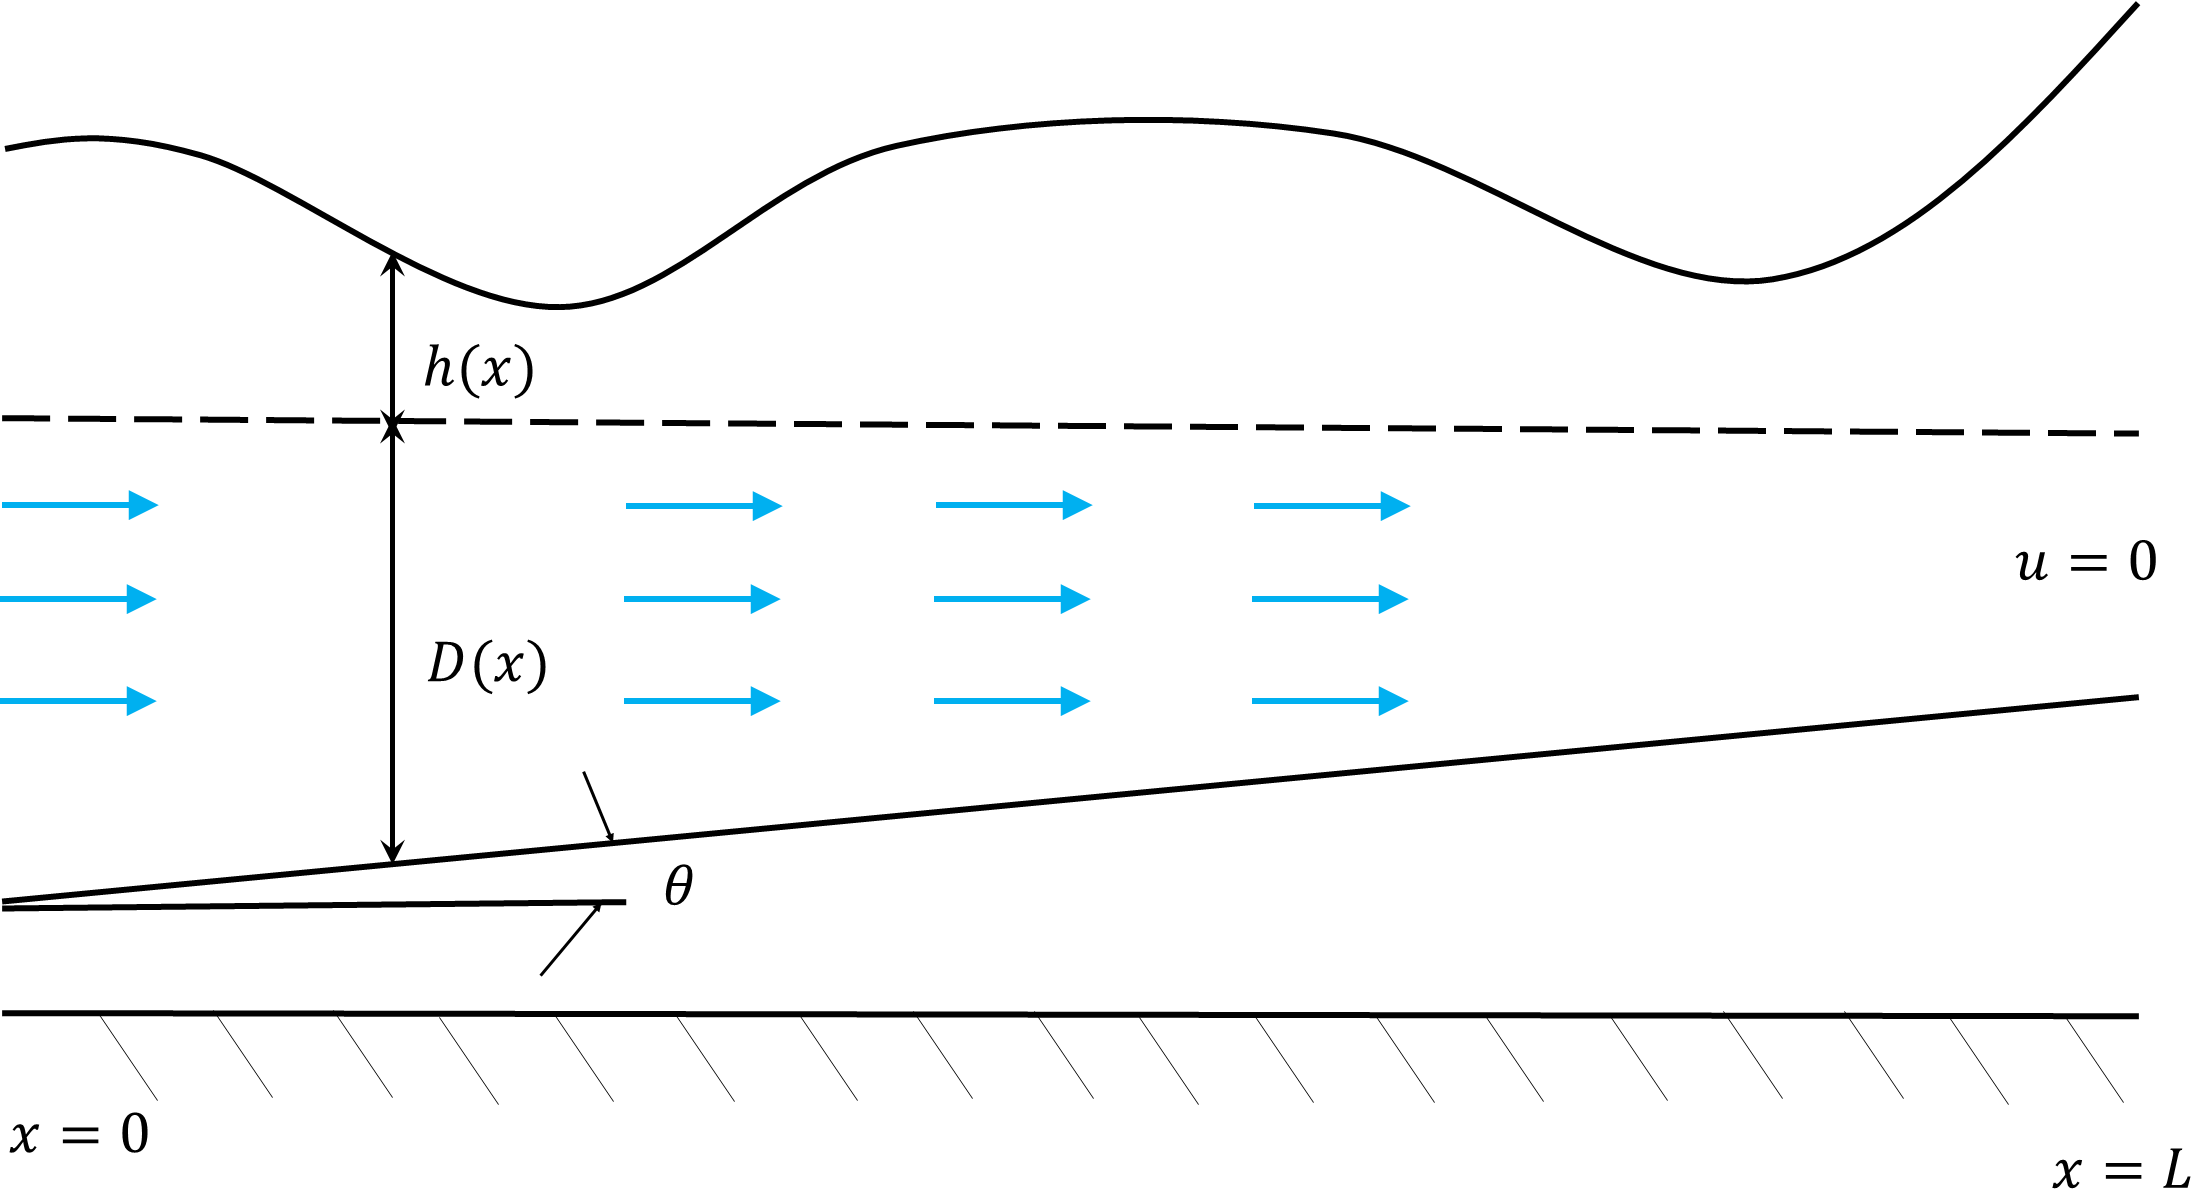
\includegraphics[scale=0.2]{figures_2/swe}
\caption{Schematic of the Tidal Water Flow}
\label{swe}
\end{figure}

The tidal water flow in a long narrow channel with varying bathymetric depth (Figure~\ref{swe}) is modeled by the Shallow Water Equations given as~\cite{verlaan1998cient}, 

\begin{equation}
\label{swe_pde}
\begin{array}{r c l}
\displaystyle \frac{\partial h}{\partial t} + D \frac{\partial u}{\partial x} + \frac{\partial D}{\partial x} u & =  & 0 \\
\displaystyle \frac{\partial u}{\partial t} + g \frac{\partial h}{\partial x} + c_f u & =  & 0 \\
h(x = 0,t) & = & h_b(t) \\
h(x ,t = 0) & = & 0 \\
u(x ,t = 0) & = & 0 \\
h(x = L ,t) & = & 0 \\
\end{array}
\end{equation}

\noindent where, $h$ denotes the water surface and $u$ is the flow velocity along the channel. The model is used to study storm surges and has been researched in details to study the effect of such surges in long narrow channels~\cite{verlaan1998cient}. The water wave is under the influence of the surge $h(0,t) = h_b(t)$. The slope is assumed as $\frac{\partial D}{\partial x} = \theta(x)$ to further simplify the system. To solve the problem, Equation~\ref{swe_pde} is discretized as per the Leendertse and Stelling scheme~\cite{verlaan1998cient,leendertse1967aspects,stelling1983construction,wesseling2009principles} as follows:

\begin{equation}
\label{swe_discrete}
\begin{array}{r c l}
\displaystyle  \frac{h_i^{k+1} - h_i^{k}}{\bigtriangleup t} + \frac{1}{2} D_i \frac{u^k_{i+\frac{1}{2}} - u^k_{i-\frac{1}{2}}}{\bigtriangleup x} + \frac{1}{2} D_i \frac{u^{k+1}_{i+\frac{1}{2}} - u^{k+1}_{i-\frac{1}{2}}}{\bigtriangleup x} +  \frac{1}{2} \theta_i \left( u^{k}_{i+\frac{1}{2}} +  u^{k+1}_{i+\frac{1}{2}} \right)  & =  & 0 \\
\displaystyle  \frac{u^{k+1}_{i+\frac{1}{2}} - u^{k}_{i+\frac{1}{2}}}{\bigtriangleup t} + \frac{1}{2} g \frac{h_{i+1}^{k} - h_i^{k}}{\bigtriangleup x}  + \frac{1}{2} g \frac{h_{i+1}^{k+1} - h_i^{k+1}}{\bigtriangleup x} + \frac{1}{2} c_f u^{k}_{i+\frac{1}{2}} + \frac{1}{2} c_f u^{k+1}_{i+\frac{1}{2}} & =  & 0 \\
h^k_0 - h_b(k \bigtriangleup t )  & =  & 0 \\
h_i^0  & =  & 0 \\
u_i^0  & =  & 0 \\
u_{N+\frac{1}{2}}^k  & =  & 0
\end{array}
\end{equation}

Equation~\ref{swe_discrete} is recast as a state space equation given by,

\begin{equation}
\label{swe_statespace}
\begin{array}{l}
\bar{D} \textbf{x}_{k+1} = \bar{A} \textbf{x}_{k} + \bar{B} \textbf{u}_k  \\
\textbf{h}_{x+1} = \bar{C} \textbf{x}_{k+1}
\end{array}
\end{equation}

where,
\begin{equation}
\label{statespace_swe}
\begin{array}{c}
\textbf{x}_k = \begin{bmatrix}
h_0^k \\ u^k_{\frac{1}{2}} \\ h_1^k \\ u^k_{1+\frac{1}{2}} \\ \vdots \\ h_N^k \\ u^k_{N+\frac{1}{2}} 
\end{bmatrix}  \hspace{5mm}
\textbf{h}_k = \begin{bmatrix}
h_0^k \\  h_1^k \\  \vdots \\ h_N^k \\ 
\end{bmatrix} \\
\bar{D} = \begin{bmatrix}
1 & 0 & 0 & 0 & 0 & \ldots & 0 \\
-\frac {g}{2\Delta x} & {\frac {1}{\Delta t}}+\frac{1}{2}\,c_{{f}} & \frac {g}{2\Delta x}  & 0 & 0 & {\ldots } & 0 \\
0 & -\frac {D_i}{2\Delta x}   & \frac {1}{\Delta t} & \frac {D_i}{2\Delta x} + \frac{1}{2}\theta_i & 0 & {\ldots } & 0 \\
\vdots & \vdots & \vdots & \vdots & \vdots & {\ldots } & \vdots \\
0 & 0 & 0 & 0 & -\frac {D_i}{2\Delta x} & \frac {1}{\Delta t} & \frac {D_i}{2\Delta x} + \frac{1}{2}\theta_i \\
0 & 0 & 0 & 0 & 0 & 0 & 1
\end{bmatrix} \\
\bar{A} = \begin{bmatrix}
0 & 0 & 0 & 0 & 0 & \ldots & 0 & 0 \\
\frac {g}{2\Delta x} & {\frac {1}{\Delta t}}-\frac{1}{2}\,c_{{f}} & -\frac {g}{2\Delta x} & 0 & 0 & {\ldots } & 0 \\
0 & \frac {D}{2\Delta x} & \frac {1}{\Delta t} & -\frac {D}{2\Delta x} - \frac{1}{2}\theta_i & 0 & {\ldots } & 0 \\
\vdots & \vdots & \vdots & \vdots & \vdots & {\ldots } & \vdots \\
0 & 0 & 0 & 0 & \frac {D}{2\Delta x} & \frac {1}{\Delta t} & -\frac {D}{2\Delta x} - \frac{1}{2}\theta_i \\
0 & 0 & 0 & 0 & 0 & 0 & 0
\end{bmatrix} \\
\bar{B} = \begin{bmatrix}
1 \\  0 \\ 0 \\ \vdots \\ 0 \\ 0
\end{bmatrix} \hspace{10mm}
\bar{C} = \begin{bmatrix}
1 & 0 & 0 & 0 & 0 & \ldots & 0  & 0 \\
0 & 0 & 1 & 0 & 0 & \ldots & 0  & 0 \\
0 & 0 & 0 & 0 & 1 & \ldots & 0  & 0 \\
\vdots & \vdots & \vdots & \vdots & \vdots & {\ldots } & \vdots & \vdots \\
0 & 0 & 0 & 0 & 0 & \ldots  & 1 & 0 \\
\end{bmatrix}
\end{array}
\end{equation}

\subsection{Results for a deterministic problem setup}
\label{deterministic}

In the deterministic test setup for Equation~\ref{swe_discrete}, the constant slope $ \theta $ in Equation~\ref{swe_statespace} is set to 0. The height of the wave at the left end is provided as an input to the equation at each time instance. The water level rises with time and the wave moves along the stretch of the channel. It then dissipates with time once the maximum height is reached. The discretized linear model in Equation~\ref{swe_statespace} is clustered by the three methods explained in Section~\ref{cluster_structure}. The adjacency matrix used in this case is $A_{sl} = \bar{D}^{-1} \bar{A}$. The parameters in Equation~\ref{swe_statespace} are assumed to be as follows:

\begin{itemize}
\item Length of the channel $L = 60$ km
\item Constant Water Depth $D = 10$ m
\item Friction constant $c_f = 0.0002$ in 1/sec
\item Total time $T = 240$ min
\end{itemize}

The discrete model in Equation~\ref{swe_discrete} is scaled using a spatial discretization of $N = 80$, with $\bigtriangleup x = L/(N+0.5)$ and a temporal discretization of $\bigtriangleup t = 300$s. Thus, the number of time steps is 80. Figure~\ref{Clustering_Types} shows the analysis of Equation~\ref{swe_statespace} using the full model and the clustered model given by the three methods of clustering. For the given test setup, Type I clustering is more effective than the other two methods of clustering. Information from one cluster is smoothly carried over to adjoining clusters via the common states. This process of information carry over is partial in Type II and absent in Type III clustering methods. 

\begin{figure}[H]
\centering
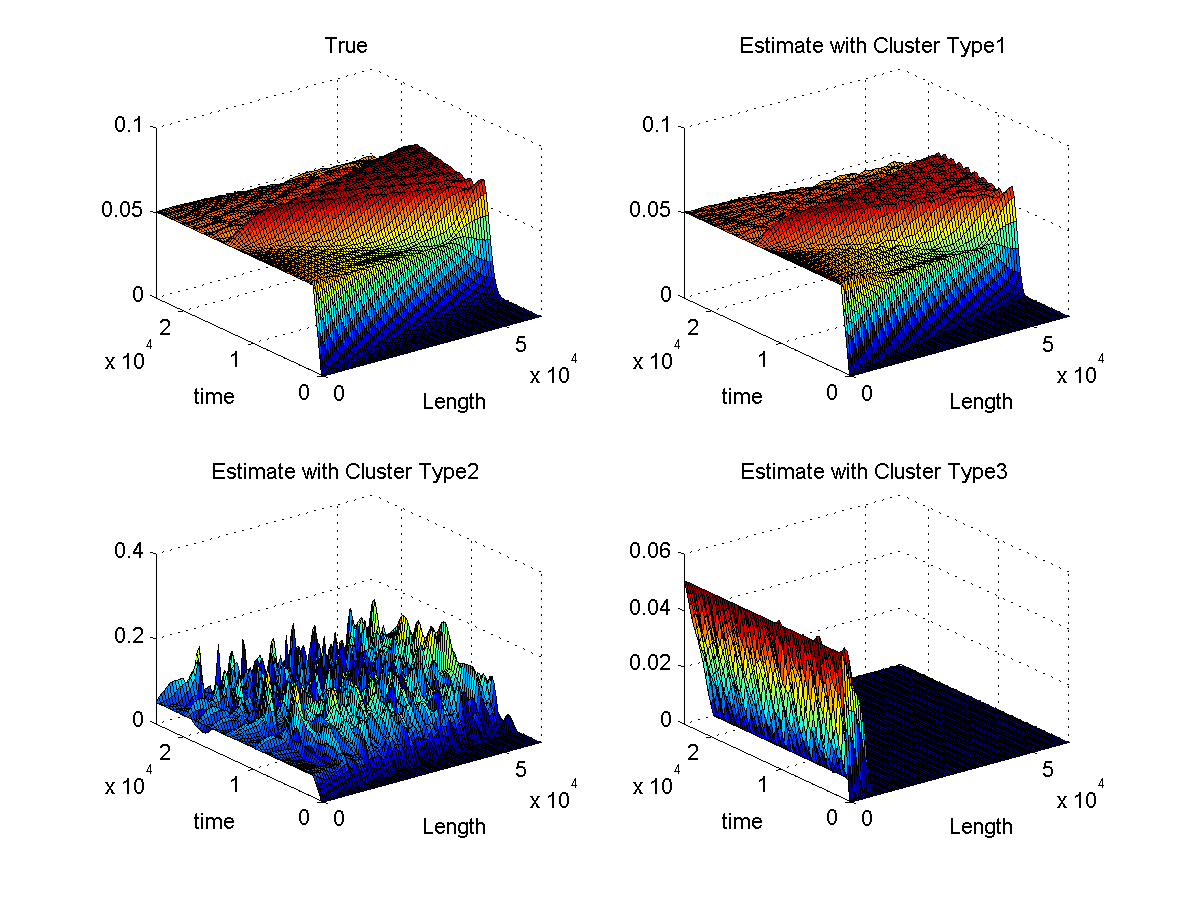
\includegraphics[scale=0.8]{figures_2/fig_comp_162_clust}
\caption{Comparison of different clustering types for a deterministic test case}
\label{Clustering_Types}
\end{figure} 

Throughout the rest of this section, Equation~\ref{swe_statespace} is solved for the same time limit of $T =  400$ mins and the length of the channel $L = 60$ km. The number of discrete spatial points $N$ has been varied from 150 to 1200, and discrete temporal points $Tstep =  T/\bigtriangleup t$ has been ranged from 60 to 1200. The stability and convergence of the discrete model are tested for the above resolutions of discretization to test the accuracy of the discrete model for solving the physical system.

\subsection{Stability Conditions}
\label{stability}
The stability conditions for a discretized model of Equation~\ref{swe_pde} is defined by the Von Neumann theory~\cite{charney1950numerical}. This condition puts a restriction on the degree of discretization for Equation~\ref{swe_discrete}. To derive the condition, following non-dimensional variables are defined:

\begin{equation}
\label{dimensionless}
\begin{array}{cccc}
\displaystyle \tilde{x} = \frac{x}{L}  & \displaystyle \tilde{t} = \frac{t}{T} & \displaystyle \tilde{h} = \frac{h}{E} & \displaystyle \tilde{u} = \frac{u}{U}
\end{array}
\end{equation} 

Thereafter, the following relations are defined:

\begin{equation}
\label{relations}
\begin{array}{cccc}
\displaystyle L^2 = DgT^2 & \displaystyle E^2 = \frac{DU^2}{g}  & \displaystyle T = \frac{\beta}{c_f} & \displaystyle \frac{TU}{E} = \alpha
\end{array}
\end{equation}

Introducing Equation~\ref{dimensionless} and~\ref{relations}, Equation~\ref{swe_pde} yields the set of following dimensionless equations:

\begin{equation}
\label{swe_dim}
\begin{array}{r c l}
\displaystyle \frac{\partial \tilde{h}}{\partial \tilde{t}} +  \frac{\partial \tilde{u}}{\partial \tilde{x}} + \theta \alpha \tilde{u} & =  & 0 \\
\displaystyle \frac{\partial \tilde{u}}{\partial \tilde{t}} +  \frac{\partial \tilde{h}}{\partial \tilde{x}} + \beta \tilde{u} & =  & 0 \\
\end{array}
\end{equation}

The solution to Equation~\ref{swe_dim} is expressed in terms of discrete Fourier modes as,

\begin{equation}
\label{fourier}
\begin{array}{l}
\tilde{h}_{i}^{k} = E^k \exp(j k_x i \bigtriangleup x) \\
\tilde{u}_{i+\frac{1}{2}}^{k} = U^k \exp(j k_x (i+\frac{1}{2}) \bigtriangleup x)
\end{array} \hspace{5mm} j^2 = -1
\end{equation}

Putting the expression for $\tilde{h}_{i}^{k}$ and $\tilde{u}_{i+1}^{k}$ into the dimensionless form of Equation~\ref{swe_discrete}, we get:

\begin{equation}
\label{fourier_mode}
\begin{array}{l}
E^{k+1} - E^{k} = -j \frac{\bigtriangleup t}{\bigtriangleup x} (U^{k} + U^{k+1}) \sin \left( \frac{k_x \bigtriangleup x}{2} \right) - \theta \alpha \frac{1}{2} \bigtriangleup t (U^{k} + U^{k+1}) \exp \left( j \frac{k_x \bigtriangleup x}{2} \right) \\
U^{k+1} - U^{k} = -j  \frac{\bigtriangleup t}{\bigtriangleup x} (E^{k} + E^{k+1}) \sin \left( \frac{k_x \bigtriangleup x}{2} \right) - \beta \frac{1}{2} \bigtriangleup t (U^{k} + U^{k+1})
\end{array}
\end{equation}

Equation~\ref{fourier_mode} is expressed in the matrix form as:

\begin{equation}
\begin{pmatrix}
E^{k+1} \\
U^{k+1}
\end{pmatrix} = 
A \begin{pmatrix}
E^{k} \\
U^{k}
\end{pmatrix}
\end{equation}

\noindent where, 
\begin{equation}
\begin{array}{l} 
A = c \resizebox{.9 \textwidth}{!}  { $ \begin{bmatrix}
-j\exp\left( j \frac{k_x \bigtriangleup x}{2} \right) \sin \left( \frac{k_x \bigtriangleup x}{2} \right) \alpha {\bigtriangleup t}^{2}\theta \bigtriangleup x
+ 2 \sin^2 \left( \frac{k_x \bigtriangleup x}{2} \right) {\bigtriangleup t}^{2} - \beta \bigtriangleup t{ \bigtriangleup x}^{2} - 2\,{ \bigtriangleup x}^{2} &  
2 \theta \alpha \bigtriangleup t \exp\left( j \frac{k_x \bigtriangleup x}{2} \right) \bigtriangleup x^2 + 4j \bigtriangleup t  \bigtriangleup x  \sin \left( \frac{k_x \bigtriangleup x}{2} \right)\\
4j \bigtriangleup t  \bigtriangleup x  \sin \left( \frac{k_x \bigtriangleup x}{2} \right) & 
-j\exp\left( j \frac{k_x \bigtriangleup x}{2} \right) \sin \left( \frac{k_x \bigtriangleup x}{2} \right) \alpha {\bigtriangleup t}^{2}\theta \bigtriangleup x  +  2 \sin^2 \left( \frac{k_x \bigtriangleup x}{2} \right) {\bigtriangleup t}^{2} + \beta \bigtriangleup t{ \bigtriangleup x}^{2} - 2\,{ \bigtriangleup x}^{2}
\end{bmatrix}$  } \\
c = \displaystyle \frac{1}{j\exp\left( j \frac{k_x \bigtriangleup x}{2} \right) \sin \left( \frac{k_x \bigtriangleup x}{2} \right) \alpha {\bigtriangleup t}^{2}\theta \bigtriangleup x
-2 \sin^2 \left( \frac{k_x \bigtriangleup x}{2} \right) {\bigtriangleup t}^{2}-\beta \bigtriangleup t{ \bigtriangleup x}^{2}-2\,{ \bigtriangleup x}^{2}
} 
\end{array} 
\end{equation}
By Von Neumann theory of stability analysis~\cite{charney1950numerical}, for a given resolution of spatio-temporal discretization or a combination of  $\bigtriangleup x$ and $\bigtriangleup t$, the system is stable if the norm of the matrix $A$ is less than 1. The discrete model in Equation~\ref{swe_discrete} has been found to be stable for all the combinations for $N$ and $\bigtriangleup t$ that have been chosen in subsection~\ref{deterministic}. 

\subsection{Convergence Analysis}

Once the discrete model is determined to be stable for a varying resolutions of discretization, the convergence analysis is performed. The discrete model is supposed to converge to the exact solution with increase in resolution. Since there is no analytic solution available, a very high resolution discretization with $N = 3200$ and $\bigtriangleup t = 15$s is chosen. The true solution for the height of the water level is given by a  $1601 \times 3201$  matrix $U_{true}$. This matrix records the height at each point along the $x$-direction for each time instance.  For a given resolution of discretization $r = (\bigtriangleup t, \bigtriangleup x)$, the same matrix $U_r$ is computed and upscaled it to the resolution of the matrix $U_{true}$ as $\hat{U}_r$. The the error rate of convergence for $r$ is calculated as,

\begin{equation}
\displaystyle \epsilon_r = \begin{Vmatrix}
\frac{U_{true} - \hat{U}_r}{U_{true}}
\end{Vmatrix}_2
\end{equation}

Figure~\ref{conv_plot} depicts the rate of convergence for different resolutions of discretization. The convergence rate decreases with increase in resolution of the discrete model.  Following the result of convergence and stability, it can be concluded that the discrete model in Equation~\ref{swe_discrete} can approximate the solution to the continuous model in Equation~\ref{swe_pde}.   

\begin{figure}[H]
\centering
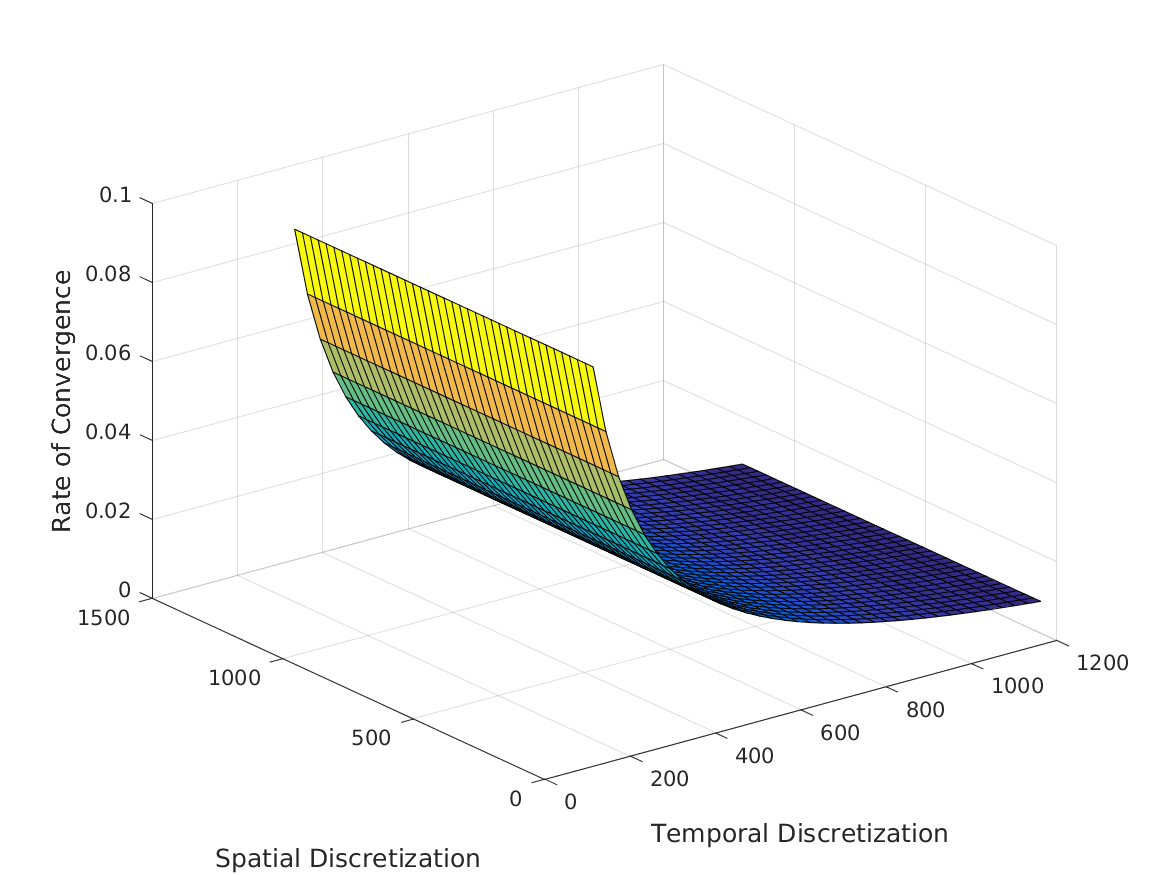
\includegraphics[width=\textwidth]{figures_2/conv_disc}
\caption{Rate of Convergence vs Discretization Resolution}
\label{conv_plot}
\end{figure}



\subsection{Cluster Length vs Resolution of Discretization}

In this section, the clusters are determined using the different methods of clustering discussed in Section~\ref{cluster_structure} for the 1-D shallow water equation~\ref{swe_discrete} to give a better physical interpretation of the state-space clusters. The state space matrix $D^{-1} A$ (Equation~\ref{statespace_swe}) is is used for clustering purpose. It is to be noted that for a given discrete point $x_k$ along the spatial domain, there are two state variables $u_i$ and $h_{i+\frac{1}{2}}$. The clustering on the $D^{-1} A$ gives us the association vectors $\textbf{z}_j$'s of the state space $\textbf{x}$ in $m$ clusters, as discussed in Section~\ref{cluster_structure}. To have a useful insight into the physical meaning of the clusters, the length of the first cluster has been chosen as the subject of interest. The length of the first cluster is given as,
\begin{equation}
\mathcal{L}_1 = \displaystyle \frac{\sum_{i=1}^{2(N+1)} \mathbb{I}_1(z_{1i}) }{2(N+1)} L \hspace{6mm} \mathbb{I}_1(z_{1i}) = \begin{cases}
1 & z_{1i} = 1 \\ 0 & \text{otherwise }
\end{cases}
\end{equation} 

The length $\mathcal{L}_1$ in kilometer represents the physical space along the channel length. Since, both $D$ and $A$ are functions of $\bigtriangleup t$ and $\bigtriangleup x$, it can be assumed that $\mathcal{L}_1$ is also a function of both $\bigtriangleup t$ and $\bigtriangleup x$.  Variation in the cluster lengths with different resolutions of discretizations is illustrated in Figures~\ref{clustlength_1} and~\ref{clustlength_2}.

\begin{figure}[H]
\centering
\begin{subfigure}[b]{0.4\textwidth}
\centering
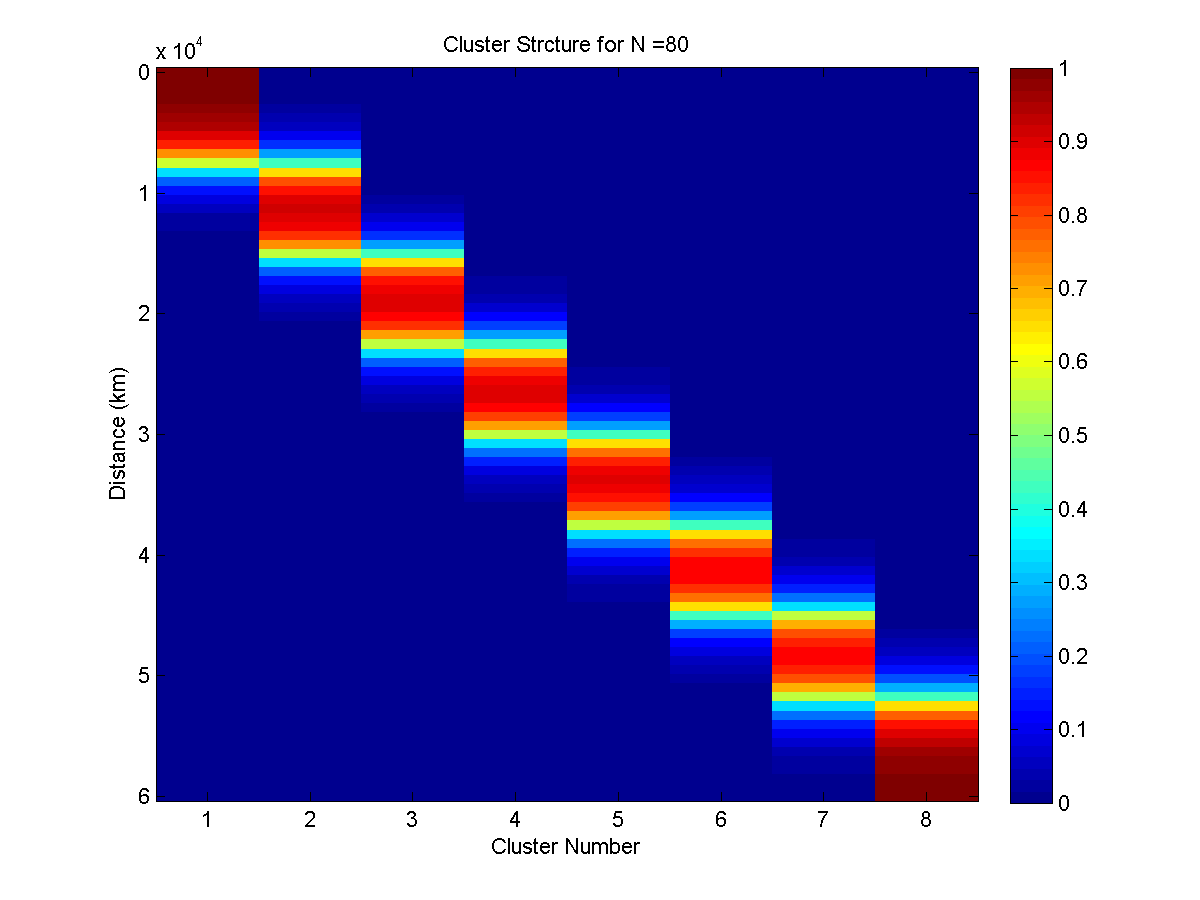
\includegraphics[width=\textwidth]{figures_2/fig_cluster_162_60_300}
\caption{Cluster Structure with N = 80}
\label{clust_N_80}
\end{subfigure}
\begin{subfigure}[b]{0.4\textwidth}
\centering
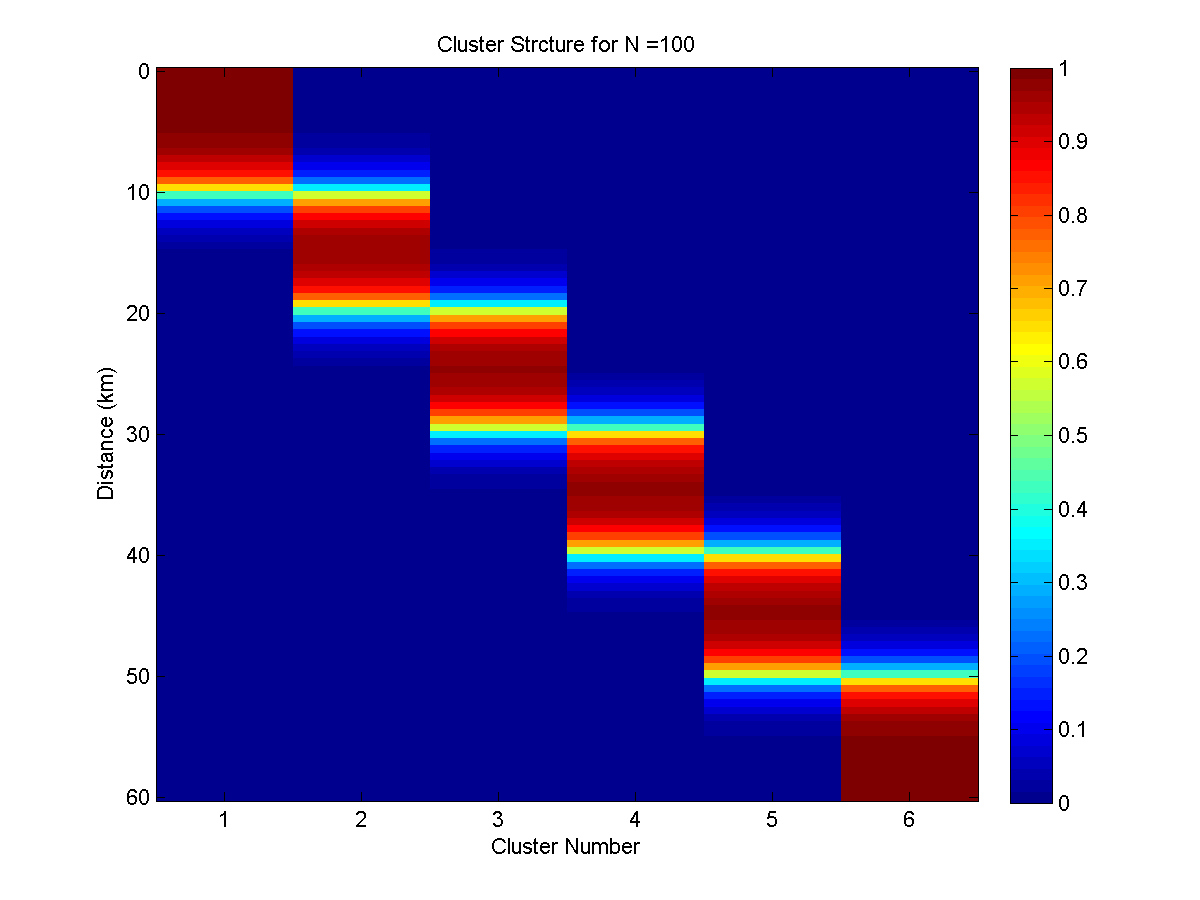
\includegraphics[width=\textwidth]{figures_2/fig_cluster_202_60_300}
\caption{Cluster Structure with N = 100}
\label{clust_N_100}
\end{subfigure}  \\
\begin{subfigure}[b]{0.4\textwidth}
\centering
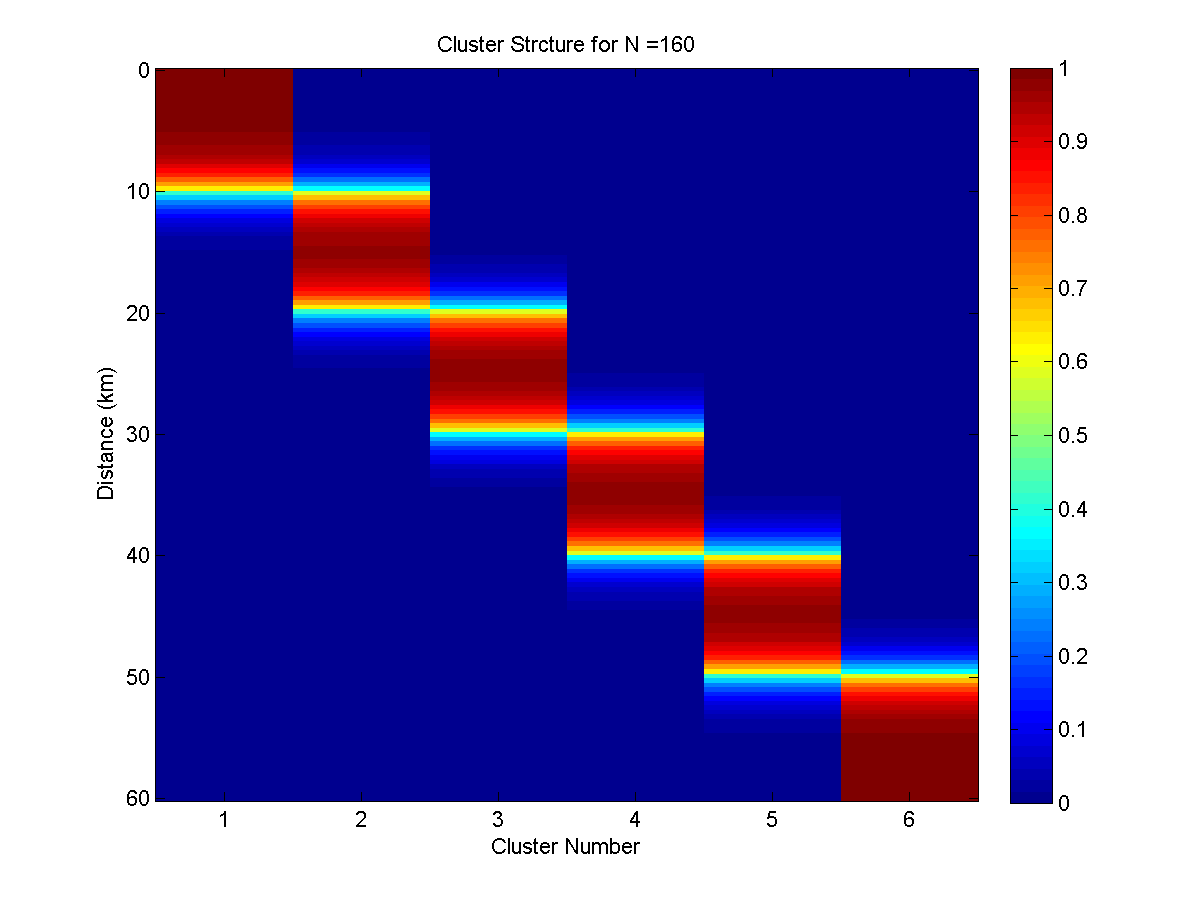
\includegraphics[width=\textwidth]{figures_2/fig_cluster_322_60_300}
\caption{Cluster Structure with N = 160}
\label{clust_N_160}
\end{subfigure}   
\begin{subfigure}[b]{0.4\textwidth}
\centering
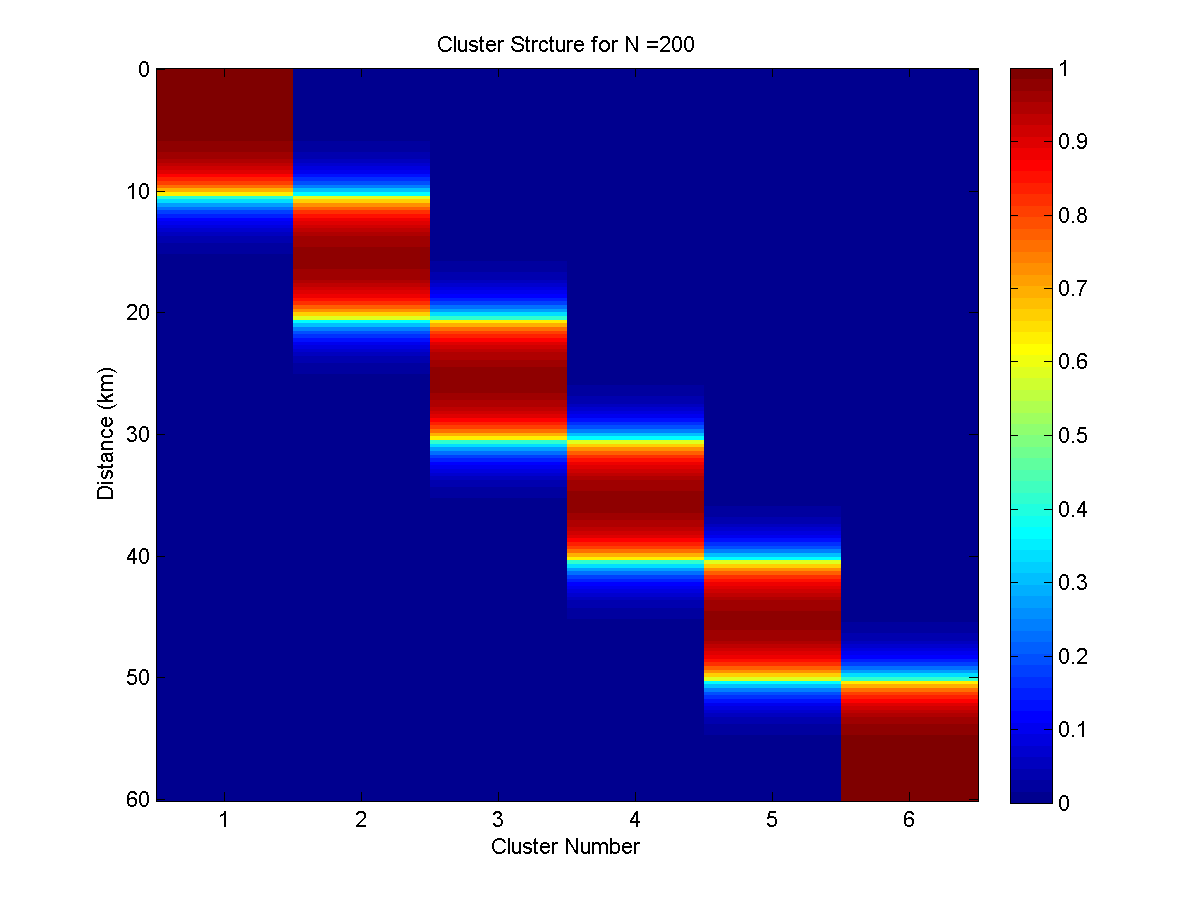
\includegraphics[width=\textwidth]{figures_2/fig_cluster_402_60_300}
\caption{Cluster Structure with N = 200}
\label{clust_N_200}
\end{subfigure}
\caption{Variation of Cluster length with varying spatial discretization and constant temporal discretization of $\bigtriangleup t = 300$s}
\label{clustlength_1}
\end{figure}

Figure~\ref{clustlength_1} shows the variation of the cluster length by varying $N = 80$ to $200$ for a constant $\bigtriangleup = 300$ s. The plots show that the cluster length is almost constant for a given $\bigtriangleup t$ and is unaffected by the change in $N$. The cluster lengths represent the physical space in which the waves can travel for a given time independent of another cluster.  This length is bound to change with an increase in $\bigtriangleup t$ or decrease in  $Tstep$.  

\begin{figure}[H]
\centering
\begin{subfigure}[b]{0.4\textwidth}
\centering
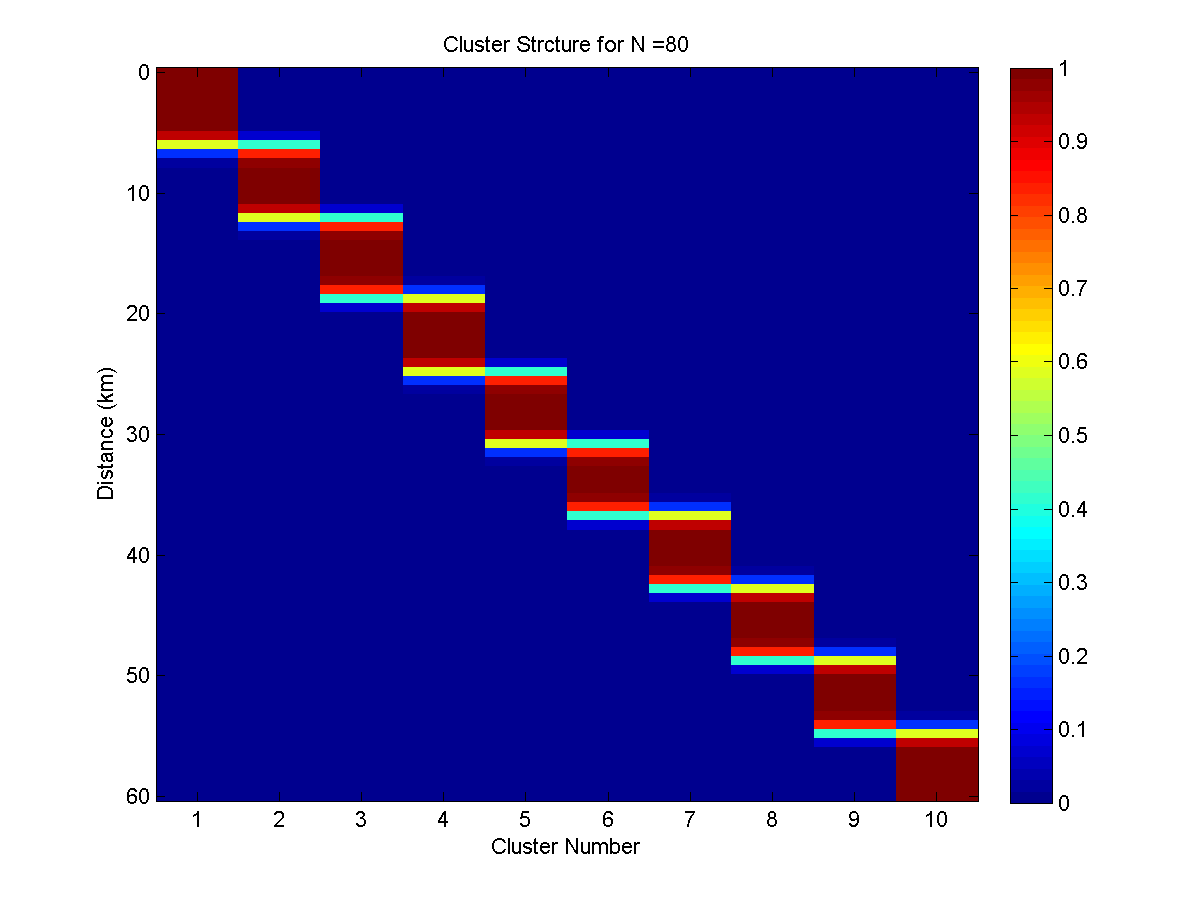
\includegraphics[width=\textwidth]{figures_2/fig_cluster_162_60_75}
\caption{Cluster Structure with $dt = 75$}
\label{clust_dt_75}
\end{subfigure}
\begin{subfigure}[b]{0.4\textwidth}
\centering
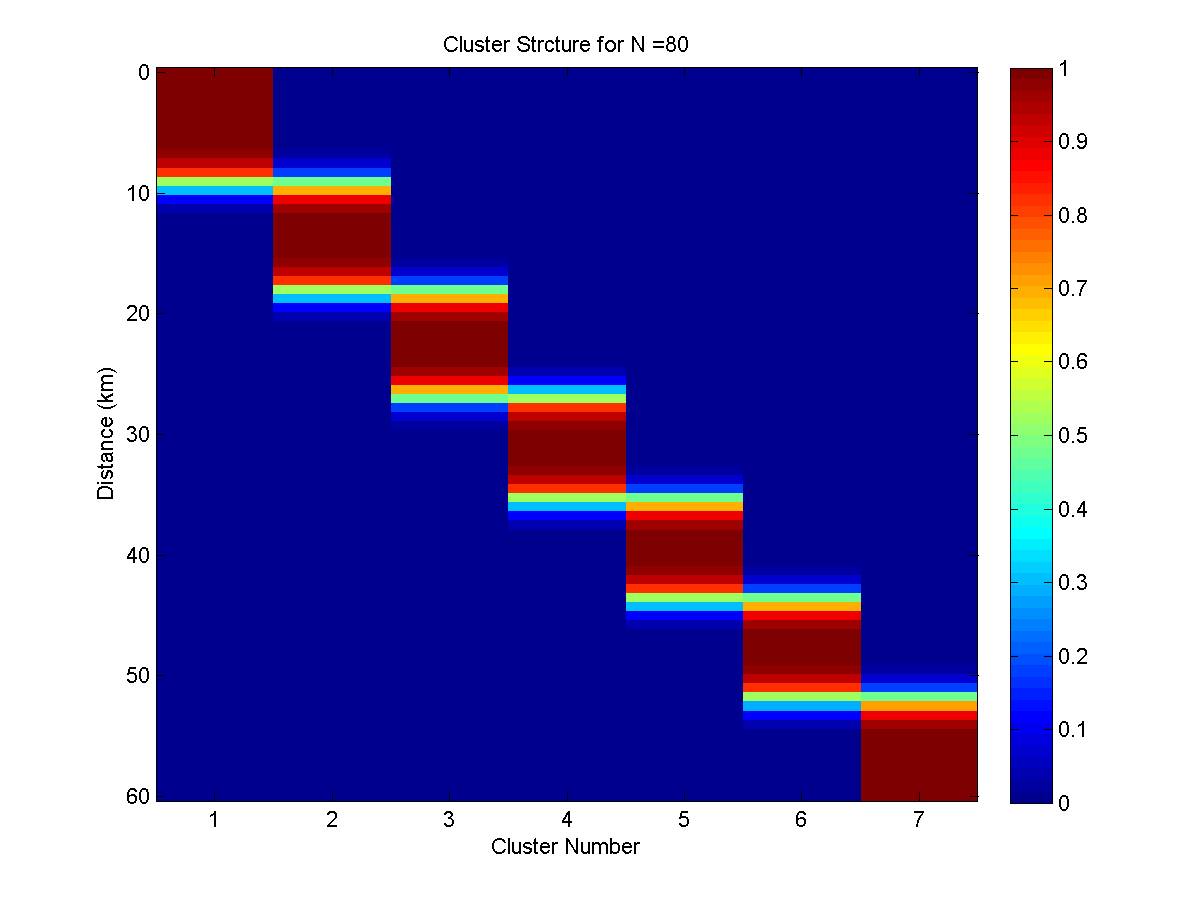
\includegraphics[width=\textwidth]{figures_2/fig_cluster_162_60_150}
\caption{Cluster Structure with $dt = 150$}
\label{clust_dt_150}
\end{subfigure}  \\
\begin{subfigure}[b]{0.4\textwidth}
\centering
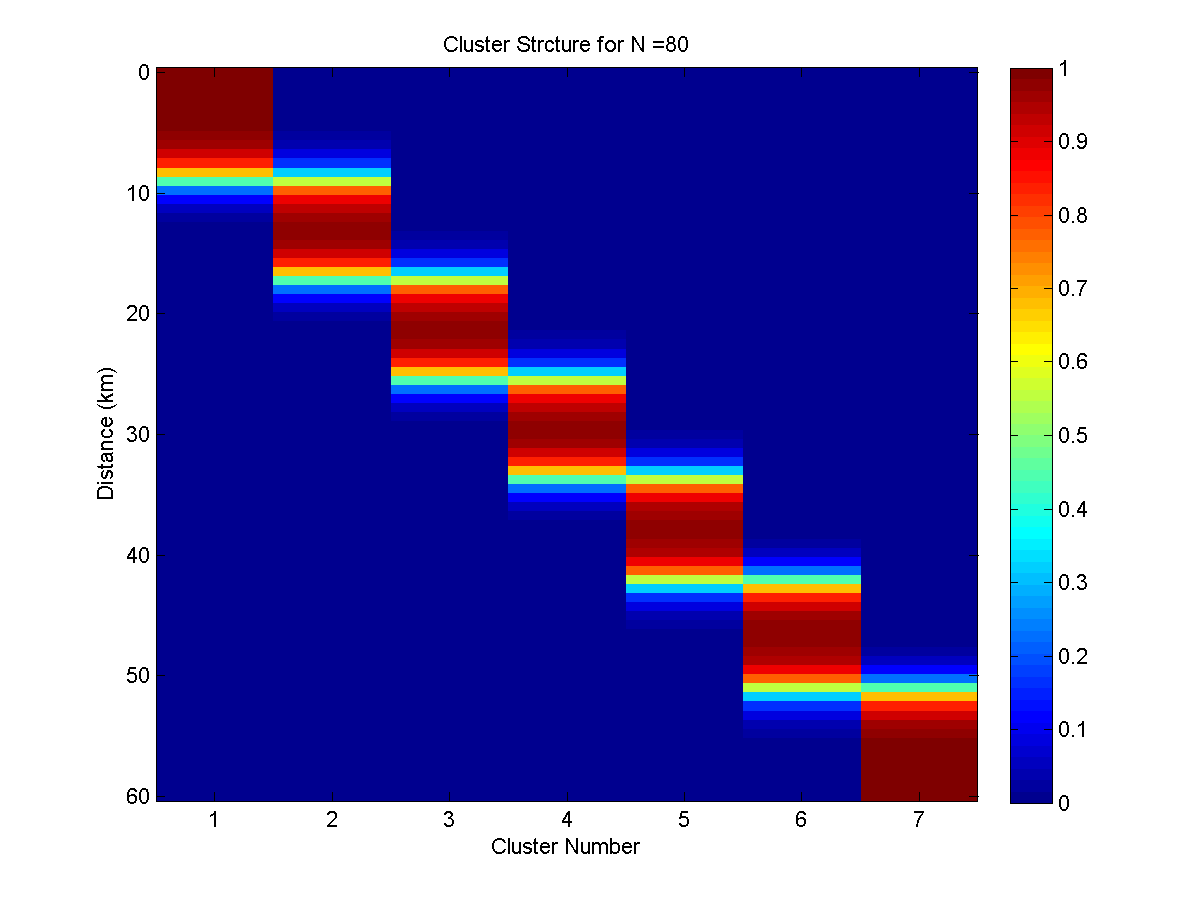
\includegraphics[width=\textwidth]{figures_2/fig_cluster_162_60_225}
\caption{Cluster Structure with $dt = 225$}
\label{clust_dt_225}
\end{subfigure}   
\begin{subfigure}[b]{0.4\textwidth}
\centering
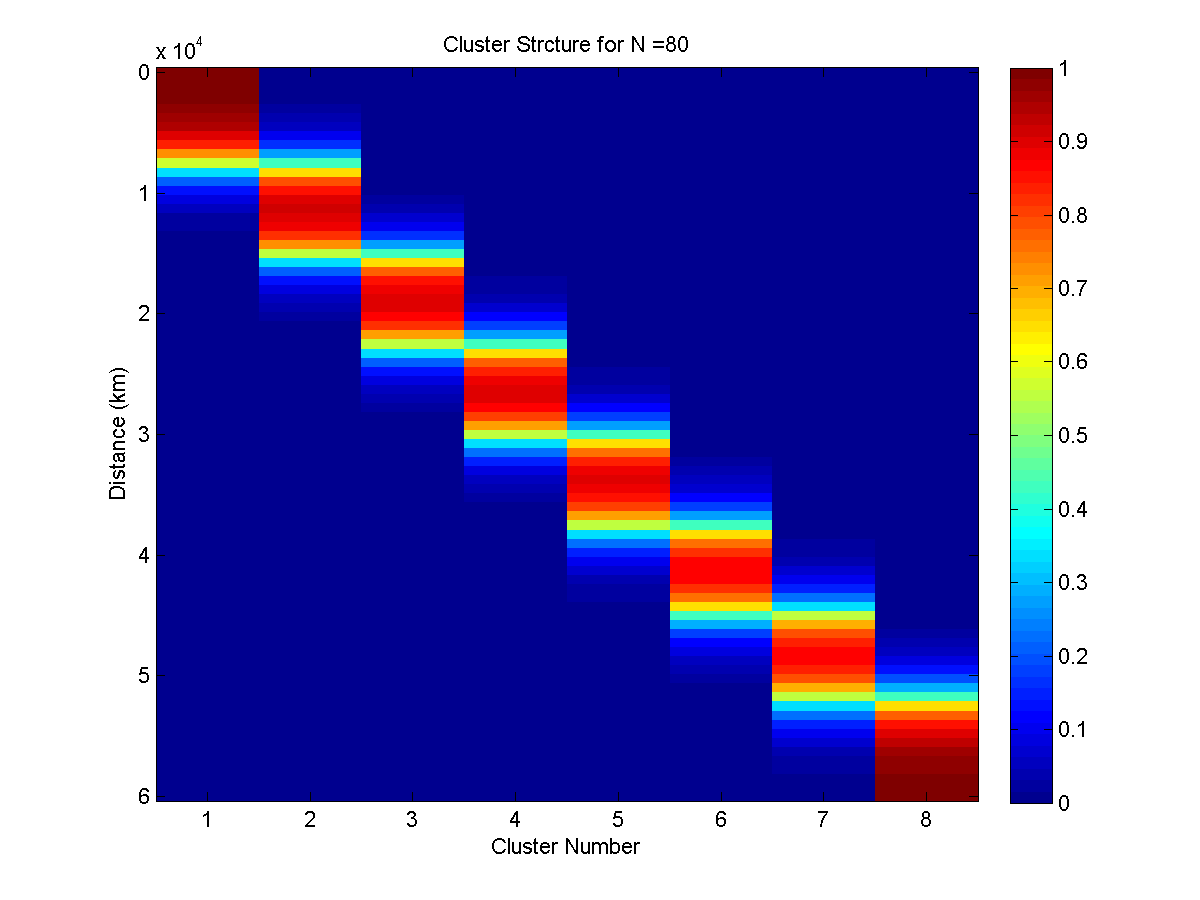
\includegraphics[width=\textwidth]{figures_2/fig_cluster_162_60_300}
\caption{Cluster Structure with $dt = 300$}
\label{clust_dt_300}
\end{subfigure}
\caption{Variation of Cluster length with constant spatial discretization $N = 80$ and varying temporal discretization}
\label{clustlength_2}
\end{figure}

Figure~\ref{clustlength_2} shows a very small variation in the values of $\mathcal{L}_1$ by varying $\bigtriangleup =  75$ to $300$s  for a constant $N = 80$. The plots show that the cluster length varies with different values of $\bigtriangleup t$. Detailed variation of the length $\mathcal{L}_1$ with change in $r$ is shown in Figure~\ref{clustlength_plot}. This analysis provides an insight into the physical meaning of the clusters. The clusters correspond to the decomposed domain that can be analyzed in parallel. The variation of the cluster lengths is consistent with the actual physical system. The subsequent UQ is carried out on the clustered model of Equation~\ref{swe_statespace} than the whole system. 

\begin{figure}[H]
\centering
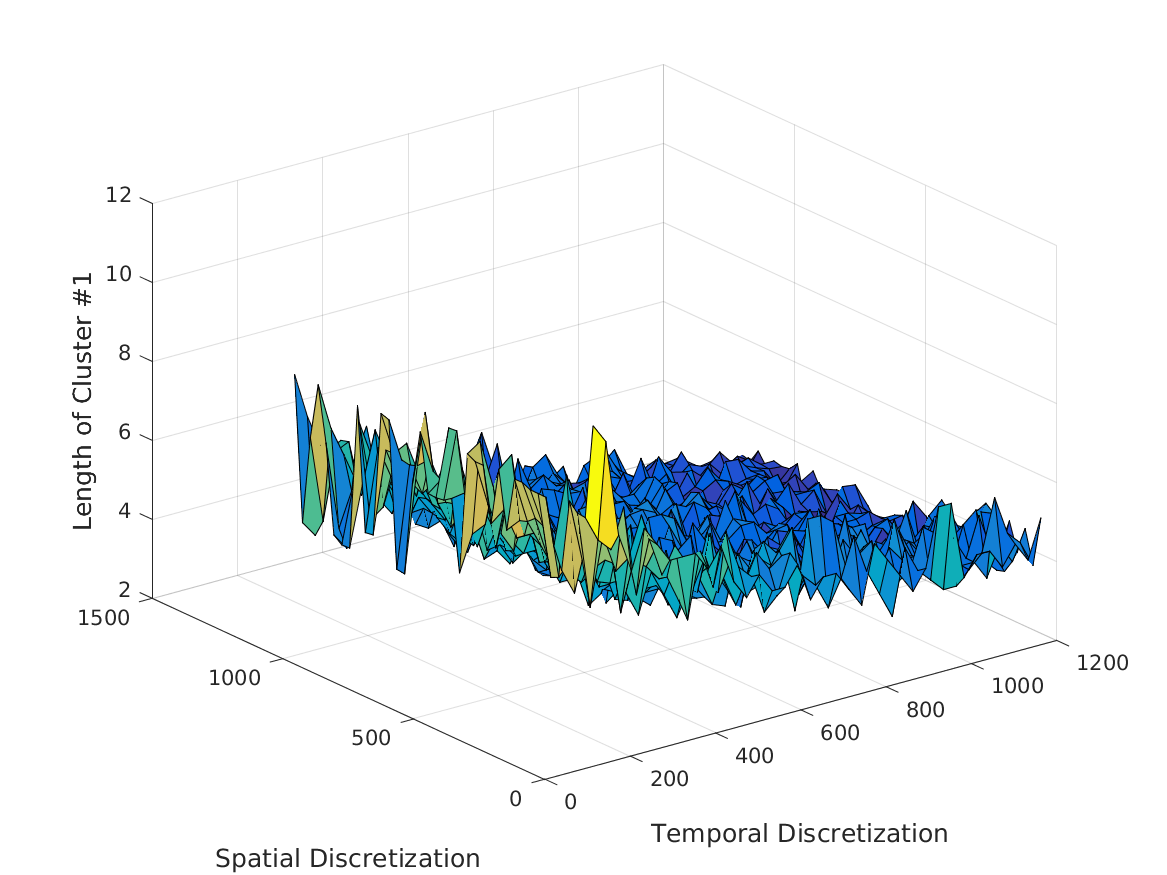
\includegraphics[width=\textwidth]{figures_2/clust_length}
\caption{Cluster Length vs Discretization Resolution}
\label{clustlength_plot}
\end{figure}


\subsection{Uncertainties associated with the model}

The bathymetric height of the system is assumed to be random for uncertainty analysis. The height and subsequently the water depth $D(x)$ is assumed to be a Gaussian random field in 1-D. The mean of $D(x)$ is assumed to have a bimodal profile shown in Figure~\ref{bathymetry} and the covariance function is assumed to be given as:

\begin{equation}
\textbf{C}(x,y) = \exp \left(-\frac{|x-y|}{a} \right)
\end{equation}

\begin{figure}[H]
\centering
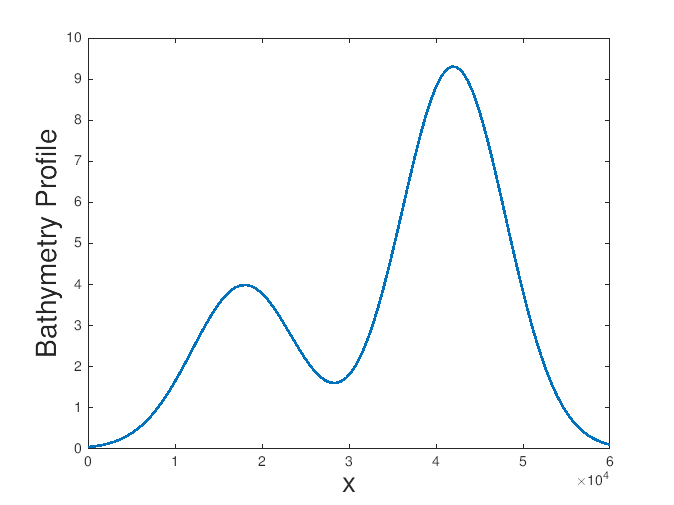
\includegraphics[scale=0.6]{figures_2/bathymetry}
\caption{Mean of the Bathymetric profile}
\label{bathymetry}
\end{figure}

$D(x)$ admits a spectral decomposition by the Karhunen-Loeve (KL) expansion as~\cite{ghanem2003stochastic}:

\begin{equation}
\label{kl_exp}
D(x)  = \mu(x) + \sum_{i=1}^\infty \sqrt{\lambda_i}\psi_i(x)D_i(x)
\end{equation}

\noindent where, $Y \sim \mathcal{N}(0,1)$ are i.i.d Gaussian random variables and $\lambda_i, \psi(x)$ are the solution to the eigenvalue problem:

\begin{equation}
\int_0^L \textbf{C}(x_1,x_2) \psi_i(x_2) dx_2 = \lambda_i \psi_i(x_1)
\end{equation}

The expansion of Equation~\ref{kl_exp} is truncated according to the decay of the eigenvalues $\lbrace \lambda_i \rbrace$s. The random field $D(x)$ is expressed in terms of the first $M$ eigenvalues as:

\begin{equation}
D(x)  = \mu(x) + \sum_{i=1}^M \sqrt{\lambda_i}\psi_i(x)D_i(x)
\end{equation} 

The eigenvalue trend for $a = 0.1L$ is depicted in Figure~\ref{eigenvalue}. This trend helps in truncating the expression of KL expansion. From the figure, $M$ can be approximated as 12. 


\begin{figure}[H]
\centering
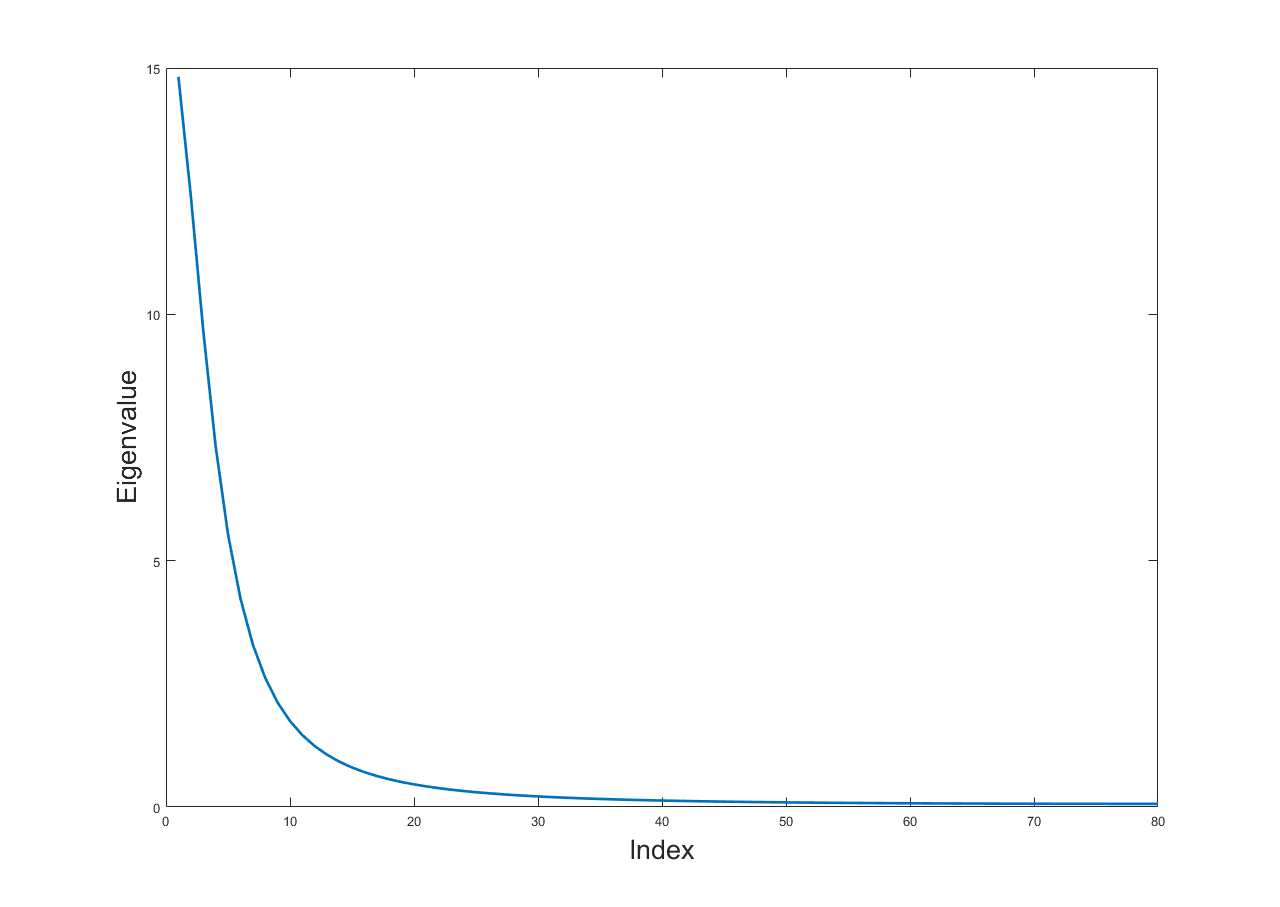
\includegraphics[scale=0.4]{figures_2/eigenvalue}
\caption{Trend of Eigenvalue for exponential covariance function with $a = 0.1L$}
\label{eigenvalue}
\end{figure}


Measurements for $\textbf{h}_{k}$ are generated using the deterministic model explained in the Section~\ref{deterministic}.  The following section details the method of clustering and UQ applied to estimate the uncertainties in the state $\textbf{h}_{k}$ and $\textbf{u}_k$.

\subsection{Clustering and Uncertainty Quantification}
 
 The state space of the model includes the discretized height of the water level $\textbf{h}_{k}$ and the velocity $\textbf{u}_k$.  The uncertainty in $\textbf{h}_k$ and $\textbf{u}_k$  is attributed to $D(x)$ and the initial state uncertainty. To cluster the state space, the statistically linearized matrix is obtained from the state-space Equation~\ref{swe_statespace}, as follows:
 
 \begin{equation}
 A_{sl}  = \int_0^L \bar{D}^{-1} (D(x)) \bar{A} (D(x)) dP_{D(x)}
\end{equation}  

For simplicity, the linearized matrix is assumed as $A_{sl} = \bar{D}^{-1} \left(E \left[ D(x) \right]\right) \bar{A} \left(E \left[ D(x) \right]\right) $. For $N=80$ and $\bigtriangleup t = 300$s, the cluster structure of $A_{sl}$ is shown in Figure~\ref{cluster_samp}. The clustering output results in five almost equal sized clusters. The clustering decomposes the 1-D domain into five overlapping domains $D_j, j=1,2,\ldots,5$. Hence, the bathymetric profile is also decomposed into five random fields. 

\begin{figure}[H]
\centering
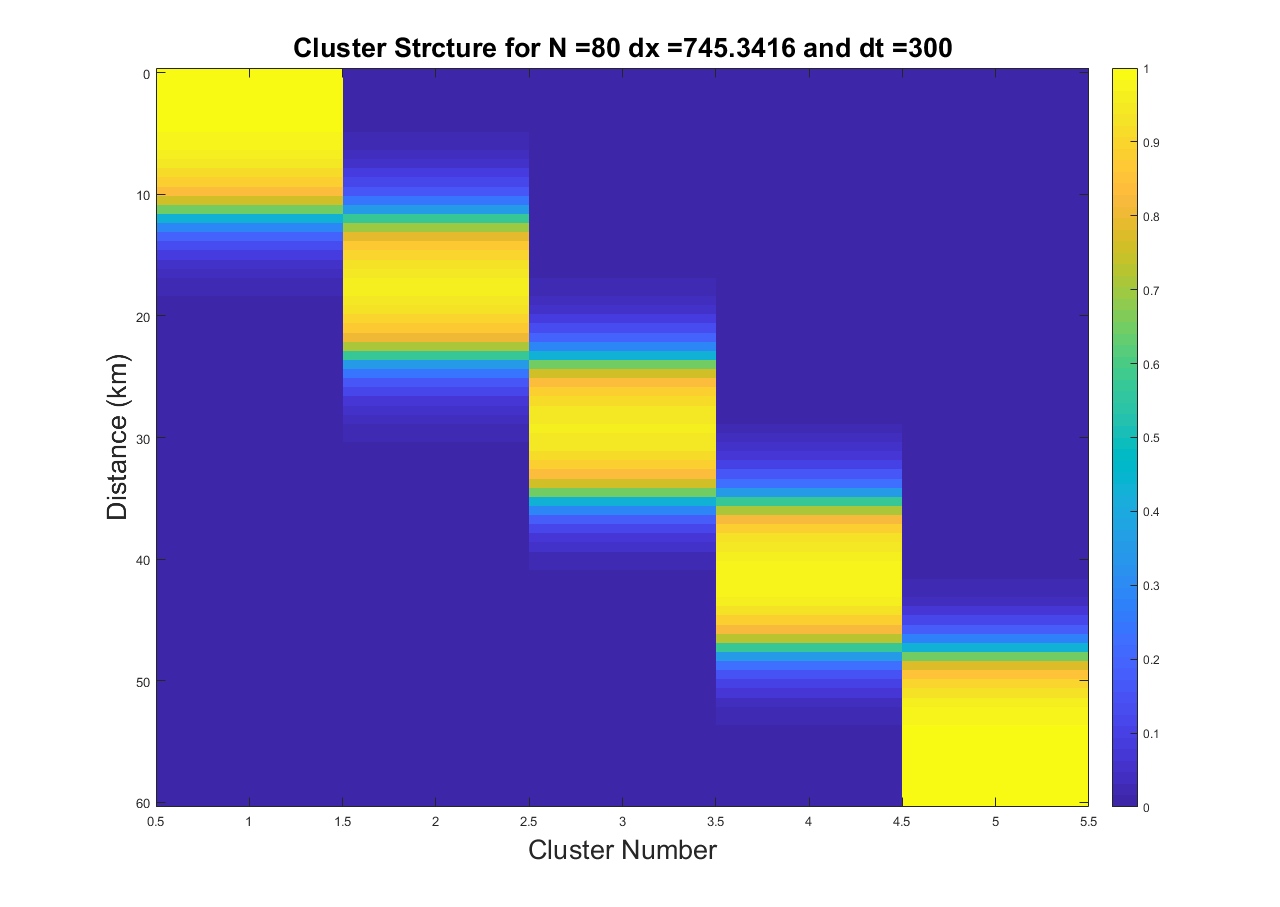
\includegraphics[scale=0.4]{figures_2/samp}
\caption{Cluster Structure for Shallow Water Model for uncertain bathymetry}
\label{cluster_samp}
\end{figure}

The effect of clustering the state space is reflected in the eigenvalue plot of the clustered random field. Figure~\ref{eigenvalue_cluster} shows the eigenvalue plot for the bathymatry random field clustered into five overlapping fields. It is observed that each cluster requires less number of eigenvalue for the truncated expansion for the random field. For each cluster $j$, the bathymetry for the domain $D_j$ can be expressed as:

\begin{equation}
D_j(x) = f(x) + \sum_{i=1}^{M_j } \sqrt{\lambda_i}\psi_i(x)D_i(x) \hspace{5 mm} x \in D_j
\end{equation}

The value of $M_j$ is approximately 4 for each cluster. This clustering reduces the total number of samples required for the random field generated by any standard quadrature method that is used to estimate high order moments. The state variables corresponding to the water level $\textbf{h}_{k}$ and the velocity $\textbf{u}_k$ are also clustered. The number of states in each cluster can be estimated from Figure~\ref{cluster_samp}.   

\begin{figure}[H]
\centering
\begin{subfigure}[b]{0.4\textwidth}
\centering
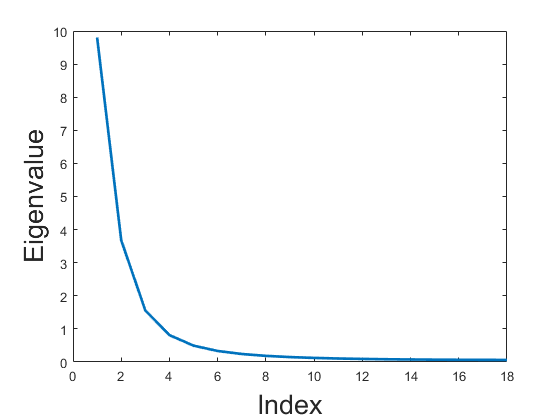
\includegraphics[width=\textwidth]{figures_2/eig1}
\caption{Cluster I}
\end{subfigure}
\begin{subfigure}[b]{0.4\textwidth}
\centering
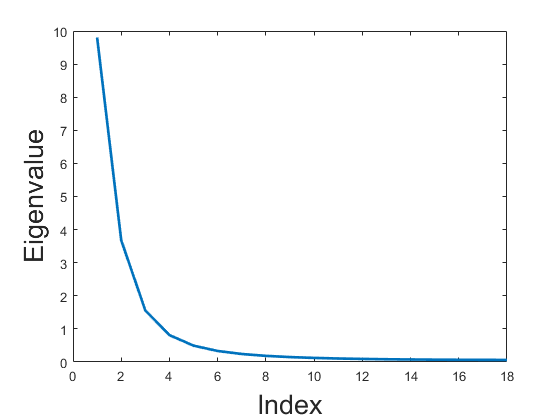
\includegraphics[width=\textwidth]{figures_2/eig2}
\caption{Cluster II}
\end{subfigure}  \\
\begin{subfigure}[b]{0.4\textwidth}
\centering
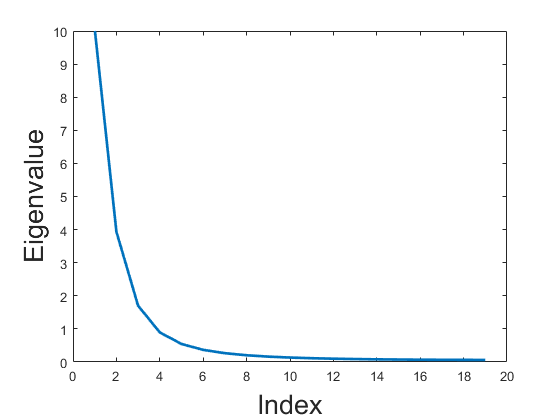
\includegraphics[width=\textwidth]{figures_2/eig3}
\caption{Cluster III}
\end{subfigure}   
\begin{subfigure}[b]{0.4\textwidth}
\centering
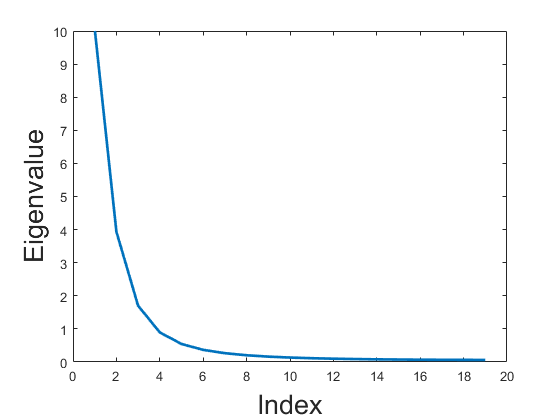
\includegraphics[width=\textwidth]{figures_2/eig4}
\caption{Cluster IV}
\end{subfigure}   \\
\begin{subfigure}[b]{0.4\textwidth}
\centering
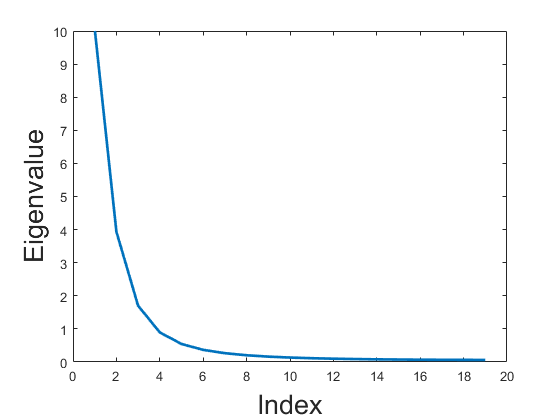
\includegraphics[width=\textwidth]{figures_2/eig5}
\caption{Cluster V}
\end{subfigure}   
\caption{Eigenvalue plot for the bathymetry random field clustered into 5 overlapping fields}
\label{eigenvalue_cluster}
\end{figure}


Corresponding filtering problem is solved as described in the Section~\ref{ukf_clust}. The effect of filtering is displayed by plotting the observed and estimated height with the $\pm 3\sigma$ limit. Figure~\ref{filterplot} shows the results of filtering out of noise with the availability of measurement. The Type I method of clustering outperforms the other two methods. While Type II and III are efficient in estimating the state, the accuracy in covariance estimation is relatively weak. 

\begin{figure}[H]
\centering
\begin{subfigure}[b]{0.3\textwidth}
\centering
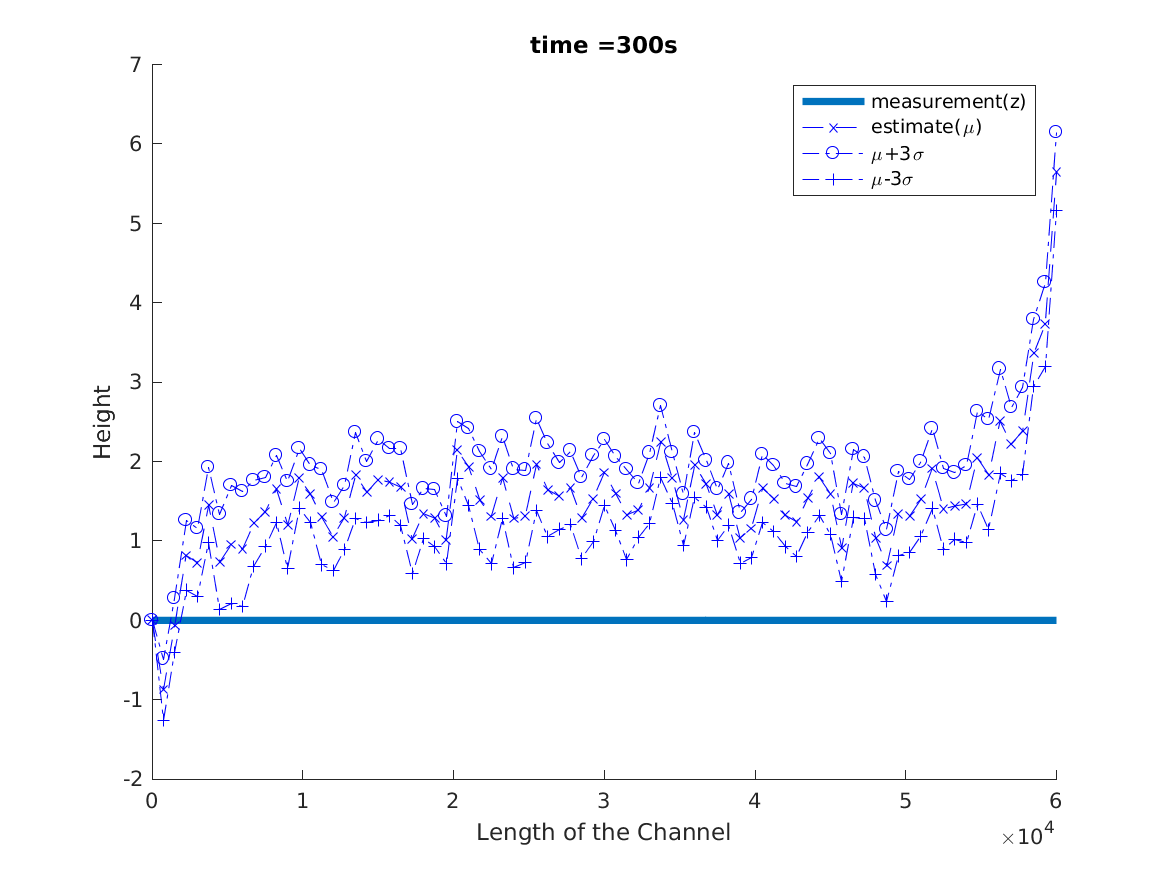
\includegraphics[width=\textwidth]{figures_2/fig11}
\caption{Cluster Technique I}
\end{subfigure}
\begin{subfigure}[b]{0.3\textwidth}
\centering
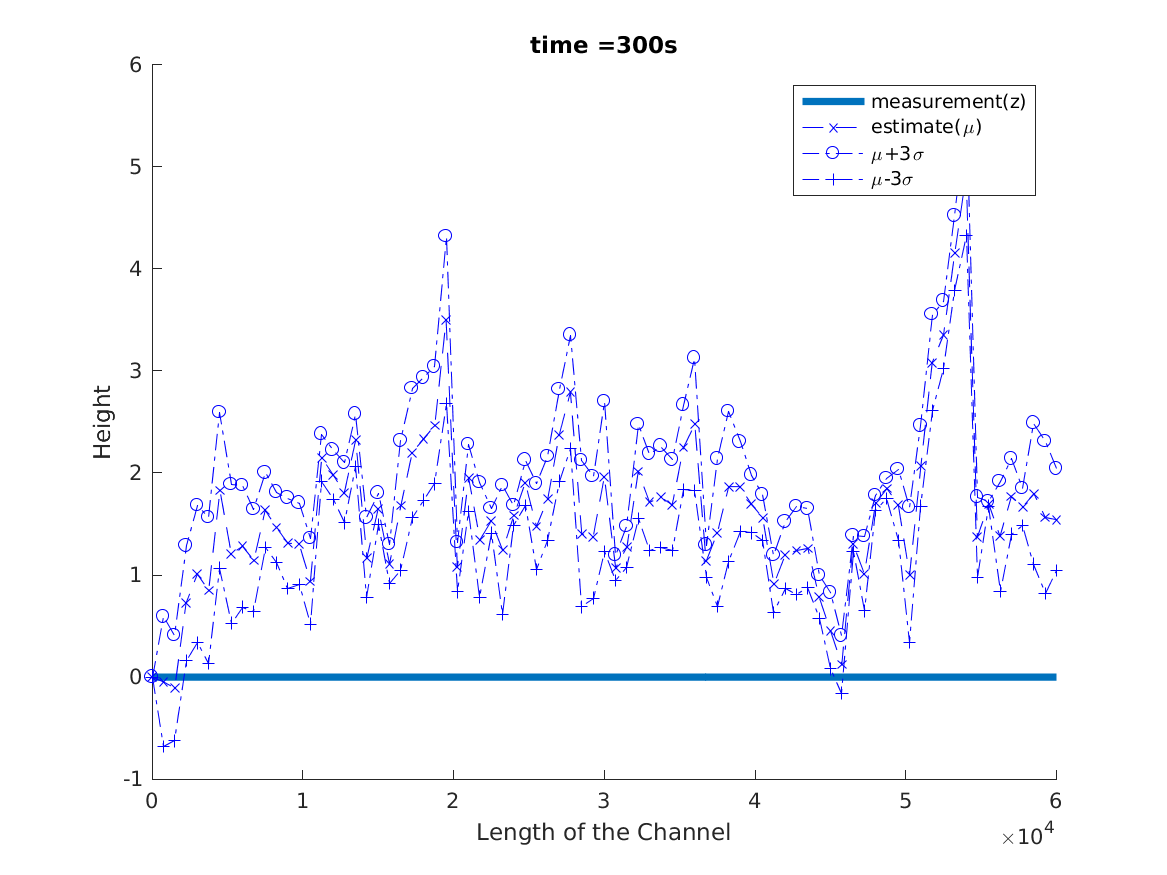
\includegraphics[width=\textwidth]{figures_2/fig21}
\caption{Cluster Technique II}
\end{subfigure} 
\begin{subfigure}[b]{0.3\textwidth}
\centering
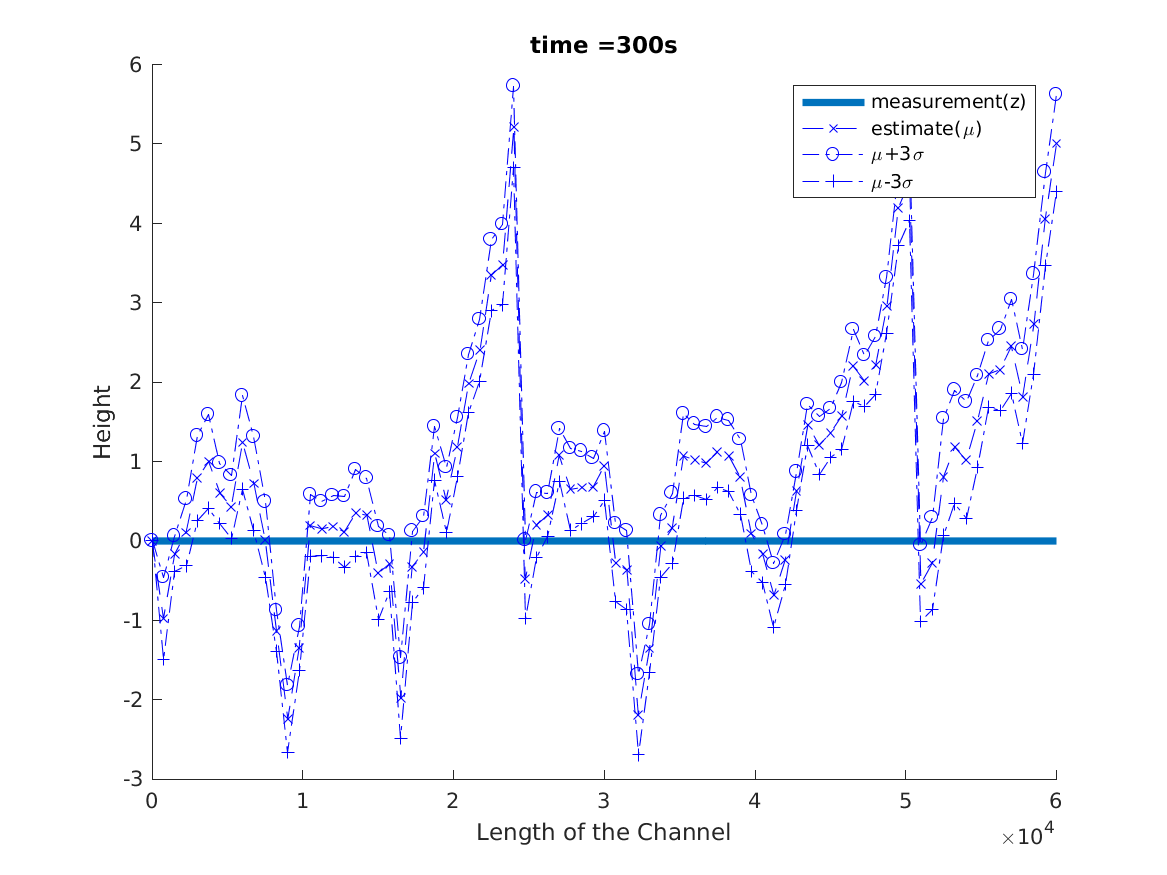
\includegraphics[width=\textwidth]{figures_2/fig31}
\caption{Cluster Technique III}
\end{subfigure}   \\
\begin{subfigure}[b]{0.3\textwidth}
\centering
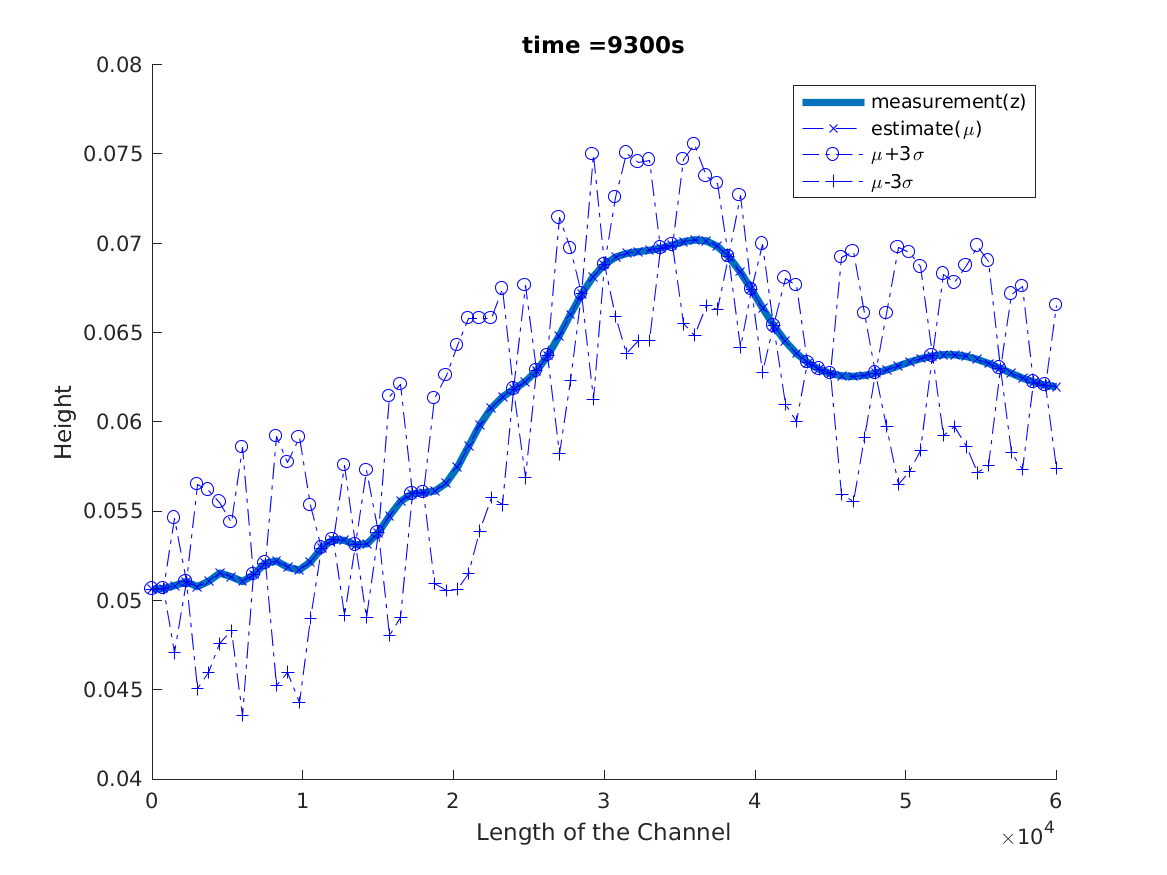
\includegraphics[width=\textwidth]{figures_2/fig131}
\caption{Cluster Technique I}
\end{subfigure}   
\begin{subfigure}[b]{0.3\textwidth}
\centering
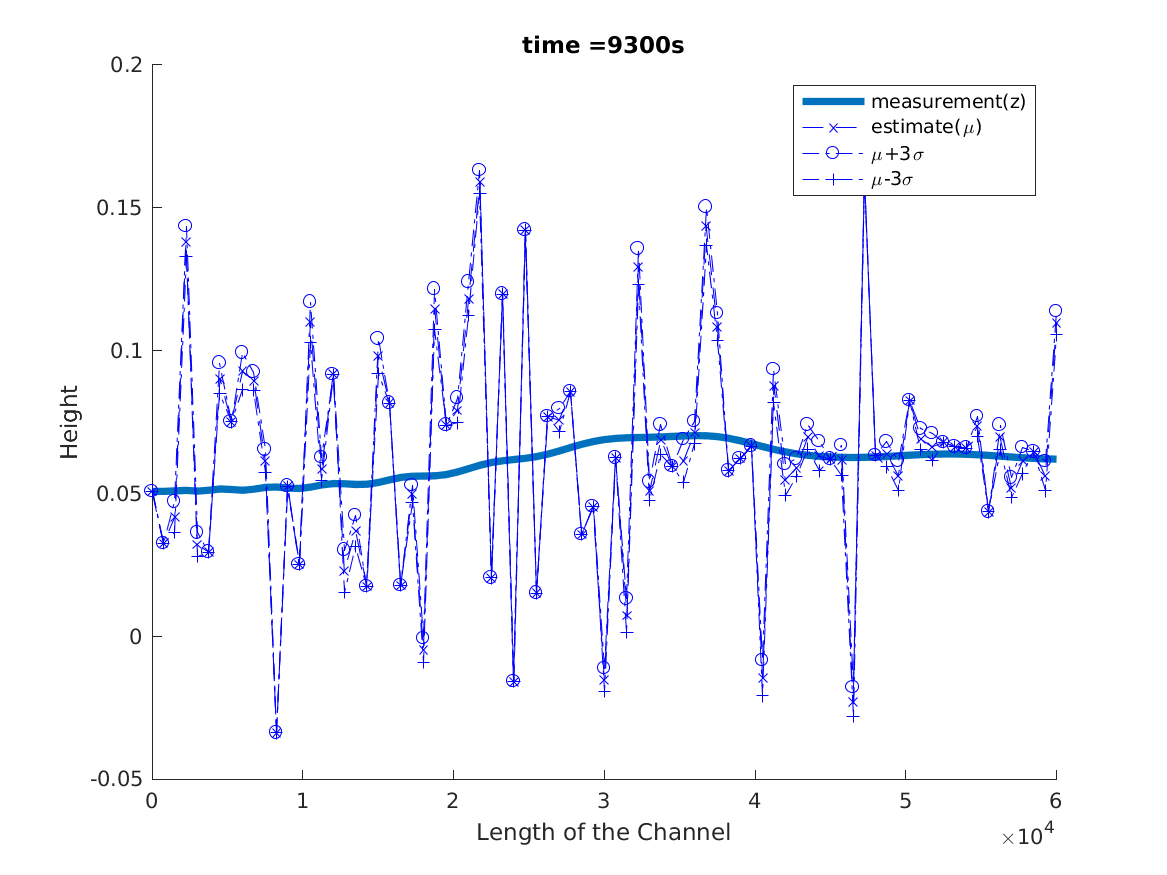
\includegraphics[width=\textwidth]{figures_2/fig231}
\caption{Cluster Technique II}
\end{subfigure}   
\begin{subfigure}[b]{0.3\textwidth}
\centering
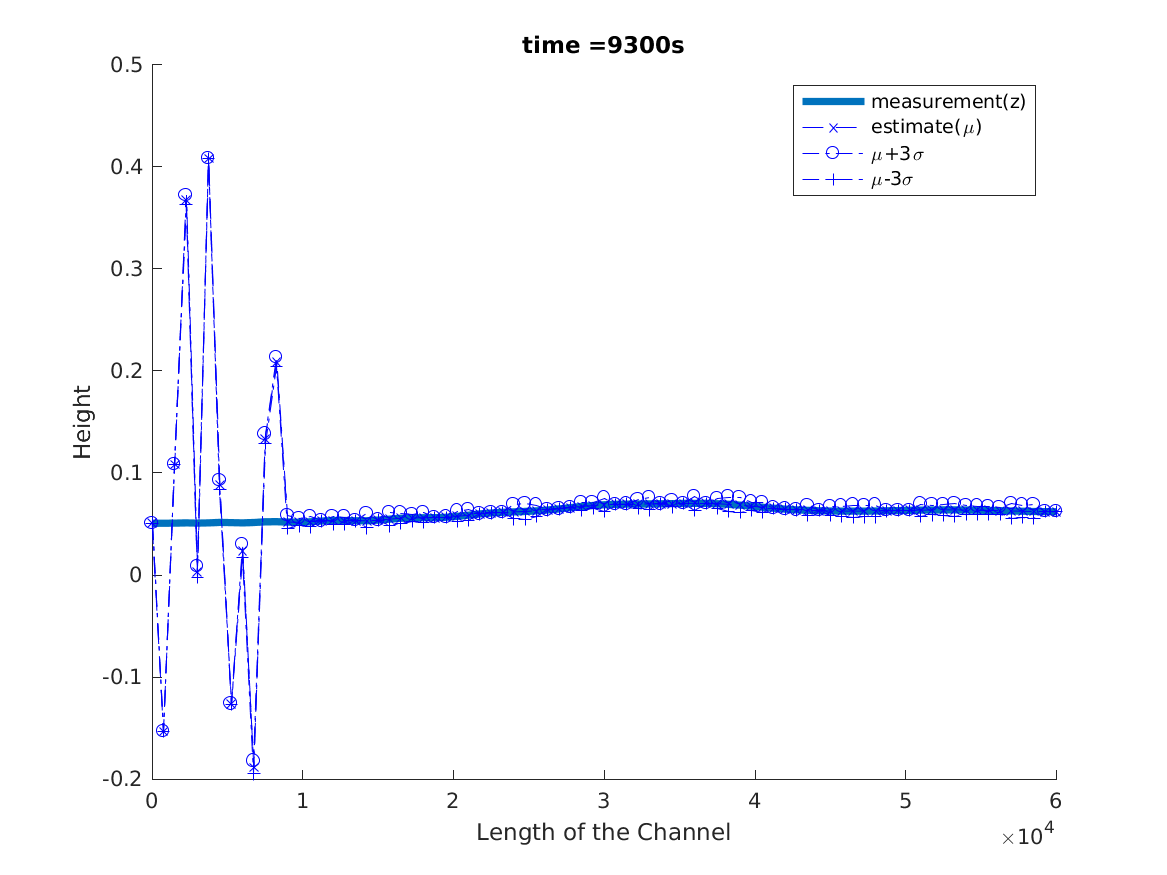
\includegraphics[width=\textwidth]{figures_2/fig331}
\caption{Cluster Technique III}
\end{subfigure} \\
\begin{subfigure}[b]{0.3\textwidth}
\centering
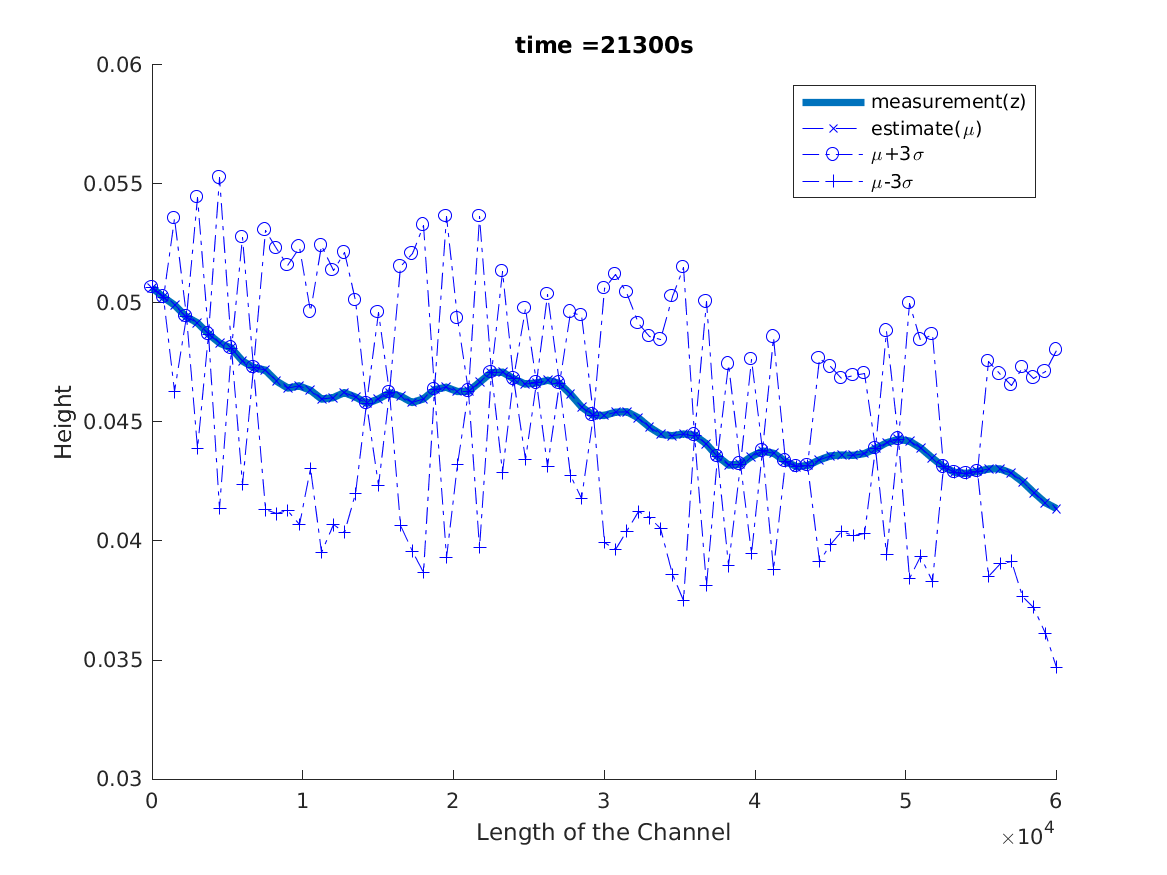
\includegraphics[width=\textwidth]{figures_2/fig171}
\caption{Cluster Technique I}
\end{subfigure}   
\begin{subfigure}[b]{0.3\textwidth}
\centering
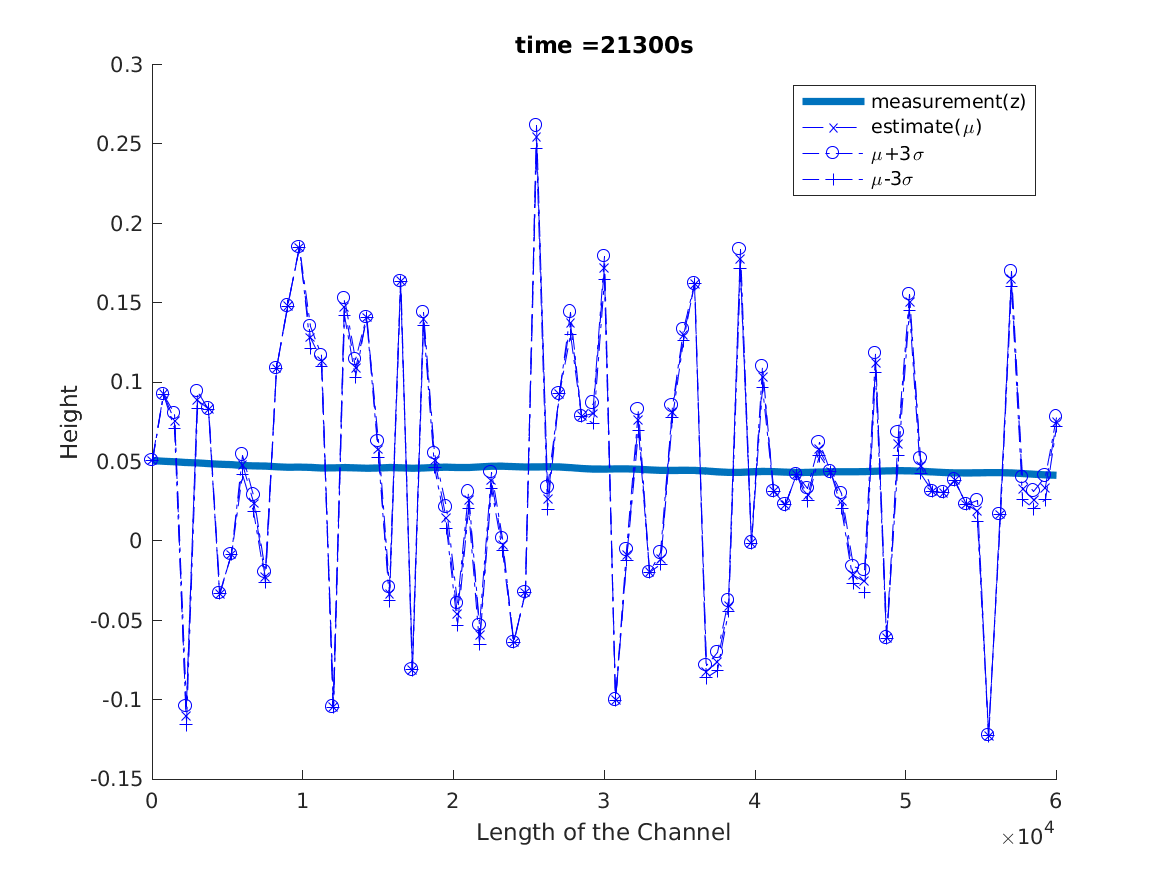
\includegraphics[width=\textwidth]{figures_2/fig271}
\caption{Cluster Technique II}
\end{subfigure}   
\begin{subfigure}[b]{0.3\textwidth}
\centering
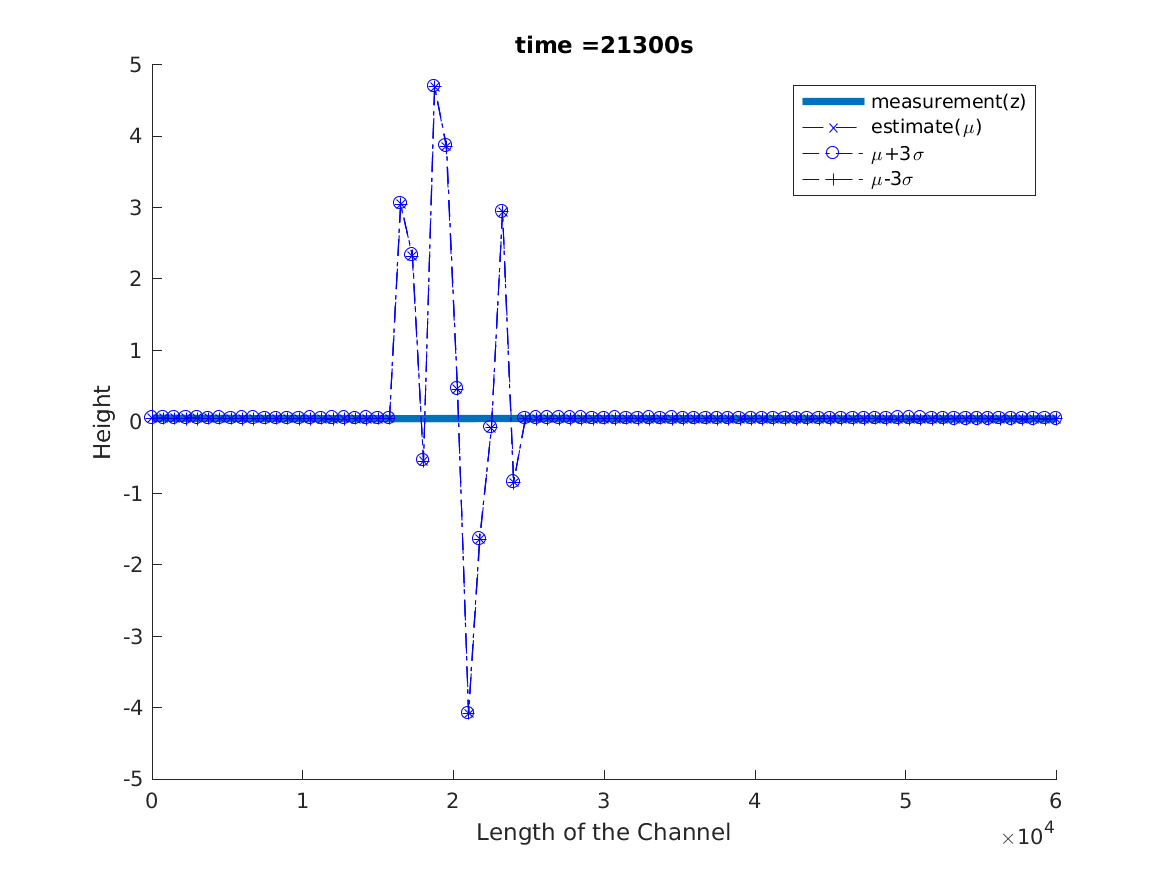
\includegraphics[width=\textwidth]{figures_2/fig371}
\caption{Cluster Technique III}
\end{subfigure}
\caption{Results of the filtering problem. The noise is filtered out with availability of measurement}
\label{filterplot}
\end{figure} 

\section{Summary}

This chapter formulates three different type of clustering methods to identify Strongly Coupled Subsystems (SCSs) in a high-dimensional uncertain dynamical systems. Two new methods of clustering the state-space are developed based on overlapping community detection algorithms. The third method uses the overlapping information and maps to a non-overlapping sets of community based on maximum participation of a state in a cluster. The decomposition of state-space based on outlined clustering methods facilitates effective UQ of a high-dimensional  system with fewer sample points with the help of any standard UQ method. 
The Type I method of linearization and clustering shows to be very effective in identifying the common states. The propagation method gives relatively lower error when compared with the two other methods. Type III clustering method gives us the highest error. The error for Type II is in between Type I and Type III. The error difference is more significant for the shallow water equation example.  The SWE model is carefully chosen for analysis in which the input at one end is propagated throughout the model. Hence, a proper communication between the clusters is essential to have the continuous flow of information in between two neighboring clusters over time. This communication is established very well by Type I method and not so well by Type II and III. 

%\textit{How to decide on the clustering method?}

The decision to choose a clustering method should be taken based on the problem and physical properties of the system. From the results, it is evident that the choice of clustering method does not create a significant difference on the results of the oscillator problems. The decision of selecting a clustering method is taken based on the balance between error estimate and the computation time required. It is evident that Type I method will need much more time since during the UQ all the states in the cluster are propagated. In Type I method the propagation equation in the cluster involves a higher number of state variables than the other methods. Type II method has the same number of cluster length as Type III, with the additional common states taken as input variables. Thus, Type II provides an accuracy close to Type I, while the time required during the UQ phase is much less. Also, Type II adjusts its cluster structure with varying coupling strengths for scalable problems. As pointed out earlier, Type II method shows similar cluster structure and hence accuracy as Type I method for high values of coupling strength $\epsilon$. Type III requires the least computation time but is also the least accurate. It has been shown in our earlier work, that for weak coupling Type III provides considerable accuracy. 

